\documentclass[twoside]{book}

% Packages required by doxygen
\usepackage{fixltx2e}
\usepackage{calc}
\usepackage{doxygen}
\usepackage[export]{adjustbox} % also loads graphicx
\usepackage{graphicx}
\usepackage[utf8]{inputenc}
\usepackage{makeidx}
\usepackage{multicol}
\usepackage{multirow}
\PassOptionsToPackage{warn}{textcomp}
\usepackage{textcomp}
\usepackage[nointegrals]{wasysym}
\usepackage[table]{xcolor}

% Font selection
\usepackage[T1]{fontenc}
\usepackage[scaled=.90]{helvet}
\usepackage{courier}
\usepackage{amssymb}
\usepackage{sectsty}
\renewcommand{\familydefault}{\sfdefault}
\allsectionsfont{%
  \fontseries{bc}\selectfont%
  \color{darkgray}%
}
\renewcommand{\DoxyLabelFont}{%
  \fontseries{bc}\selectfont%
  \color{darkgray}%
}
\newcommand{\+}{\discretionary{\mbox{\scriptsize$\hookleftarrow$}}{}{}}

% Page & text layout
\usepackage{geometry}
\geometry{%
  a4paper,%
  top=2.5cm,%
  bottom=2.5cm,%
  left=2.5cm,%
  right=2.5cm%
}
\tolerance=750
\hfuzz=15pt
\hbadness=750
\setlength{\emergencystretch}{15pt}
\setlength{\parindent}{0cm}
\setlength{\parskip}{3ex plus 2ex minus 2ex}
\makeatletter
\renewcommand{\paragraph}{%
  \@startsection{paragraph}{4}{0ex}{-1.0ex}{1.0ex}{%
    \normalfont\normalsize\bfseries\SS@parafont%
  }%
}
\renewcommand{\subparagraph}{%
  \@startsection{subparagraph}{5}{0ex}{-1.0ex}{1.0ex}{%
    \normalfont\normalsize\bfseries\SS@subparafont%
  }%
}
\makeatother

% Headers & footers
\usepackage{fancyhdr}
\pagestyle{fancyplain}
\fancyhead[LE]{\fancyplain{}{\bfseries\thepage}}
\fancyhead[CE]{\fancyplain{}{}}
\fancyhead[RE]{\fancyplain{}{\bfseries\leftmark}}
\fancyhead[LO]{\fancyplain{}{\bfseries\rightmark}}
\fancyhead[CO]{\fancyplain{}{}}
\fancyhead[RO]{\fancyplain{}{\bfseries\thepage}}
\fancyfoot[LE]{\fancyplain{}{}}
\fancyfoot[CE]{\fancyplain{}{}}
\fancyfoot[RE]{\fancyplain{}{\bfseries\scriptsize Generated by Doxygen }}
\fancyfoot[LO]{\fancyplain{}{\bfseries\scriptsize Generated by Doxygen }}
\fancyfoot[CO]{\fancyplain{}{}}
\fancyfoot[RO]{\fancyplain{}{}}
\renewcommand{\footrulewidth}{0.4pt}
\renewcommand{\chaptermark}[1]{%
  \markboth{#1}{}%
}
\renewcommand{\sectionmark}[1]{%
  \markright{\thesection\ #1}%
}

% Indices & bibliography
\usepackage{natbib}
\usepackage[titles]{tocloft}
\setcounter{tocdepth}{3}
\setcounter{secnumdepth}{5}
\makeindex

% Hyperlinks (required, but should be loaded last)
\usepackage{ifpdf}
\ifpdf
  \usepackage[pdftex,pagebackref=true]{hyperref}
\else
  \usepackage[ps2pdf,pagebackref=true]{hyperref}
\fi
\hypersetup{%
  colorlinks=true,%
  linkcolor=blue,%
  citecolor=blue,%
  unicode%
}

% Custom commands
\newcommand{\clearemptydoublepage}{%
  \newpage{\pagestyle{empty}\cleardoublepage}%
}

\usepackage{caption}
\captionsetup{labelsep=space,justification=centering,font={bf},singlelinecheck=off,skip=4pt,position=top}

%===== C O N T E N T S =====

\begin{document}

% Titlepage & ToC
\hypersetup{pageanchor=false,
             bookmarksnumbered=true,
             pdfencoding=unicode
            }
\pagenumbering{alph}
\begin{titlepage}
\vspace*{7cm}
\begin{center}%
{\Large robot\+\_\+fingers }\\
\vspace*{1cm}
{\large Generated by Doxygen 1.8.13}\\
\end{center}
\end{titlepage}
\clearemptydoublepage
\pagenumbering{roman}
\tableofcontents
\clearemptydoublepage
\pagenumbering{arabic}
\hypersetup{pageanchor=true}

%--- Begin generated contents ---
\chapter{(Tri-\/)Finger Robot Driver and Tools}
\label{index}\hypertarget{index}{}This is the documentation of the {\ttfamily robot\+\_\+fingers} package.

The source code is hosted on \href{https://github.com/open-dynamic-robot-initiative/robot_fingers}{\tt Git\+Hub}. Please also use the issue system there if you have a question or want to report a bug.

For more information, on the Tri\+Finger robot and the general architecture of the software, see also our \href{https://arxiv.org/abs/2008.03596}{\tt paper} on the open-\/source version of the Tri\+Finger robot.

\subsection*{Content }


\begin{DoxyItemize}
\item \hyperlink{md_doc_installation}{Build Instructions}
\item \hyperlink{md_doc_singularity}{About Singularity}
\item \hyperlink{md_doc_getting_started}{Getting Started}
\item \hyperlink{md_doc_hardware_testing}{Tools for Hardware Testing}
\end{DoxyItemize}

\subsection*{Links }


\begin{DoxyItemize}
\item \href{https://github.com/open-dynamic-robot-initiative/robot_fingers}{\tt Git\+Hub Repository}.
\item \href{https://github.com/open-dynamic-robot-initiative/robot_fingers/issues}{\tt Bug Tracker}.
\item This package implements a {\ttfamily Robot\+Driver} for the (Tri-\/)Finger robots based on our \href{https://open-dynamic-robot-initiative.github.io/code_documentation/robot_interfaces/docs/doxygen/html/index.html}{\tt {\ttfamily robot\+\_\+interfaces} package}. 
\end{DoxyItemize}
\chapter{Getting Started}
\label{md_doc_getting_started}
\Hypertarget{md_doc_getting_started}
This package implements a Robot\+Driver and several applications for the Tri\+Finger robots, using the \href{https://open-dynamic-robot-initiative.github.io/code_documentation/robot_interfaces/docs/doxygen/html/index.html}{\tt {\ttfamily robot\+\_\+interfaces} package}. See there for more information on the general architecture. The action and observation types for the (Tri)Finger robots are also implemented in {\ttfamily robot\+\_\+interfaces}.

We provide several \href{https://github.com/open-dynamic-robot-initiative/robot_fingers/blob/master/demos}{\tt demos} to show how to use the interface on practical examples. Good starting points are\+:


\begin{DoxyItemize}
\item \href{https://github.com/open-dynamic-robot-initiative/robot_fingers/blob/master/demos/demo_real_finger.py}{\tt demo\+\_\+real\+\_\+finger.\+py}\+: Basic example on how to control the robot using either torque or position commands. This uses only a single finger but the principle is the same for the Tri\+Finger.
\item \href{https://github.com/open-dynamic-robot-initiative/robot_fingers/blob/master/demos/demo_trifinger.py}{\tt demo\+\_\+trifinger.\+py}\+: Demo for the Tri\+Finger, moving it in a hard-\/coded choreography.
\end{DoxyItemize}

\begin{DoxyNote}{Note}
The demos are all in Python, however, you can do exactly the same using the C++ A\+PI. 
\end{DoxyNote}

\chapter{Tools for Hardware Testing}
\label{md_doc_hardware_testing}
\Hypertarget{md_doc_hardware_testing}
\subsection*{Single Finger Test }

The {\ttfamily robot\+\_\+fingers} package provides a script {\ttfamily single\+\_\+finger\+\_\+test.\+py} for testing basic functionality of a single Finger. After initialization, it holds all joints at their current position using position control. All available data is shown and constantly updated on the terminal\+:

 \subsubsection*{Running}

Start the application with the following command\+: \begin{DoxyVerb}rosrun robot_fingers single_finger_test.py
\end{DoxyVerb}


For this application, homing is done without end stops, that is the joints will simply home on the nearest encoder index without offset.

To quit simply press \char`\"{}q\char`\"{}.

\subsubsection*{Configuration}

The robot configuration used in application is found in {\ttfamily robot\+\_\+fingers/config/single\+\_\+finger\+\_\+test.\+yml}. Typically the configuration should work well, however, you may need to adjust the C\+AN ports to match the ports on which the finger is connected. 
\chapter{Build Instructions}
\label{md_doc_installation}
\Hypertarget{md_doc_installation}
We provide a Singularity image with all required dependencies to build and run the software. See \hyperlink{md_doc_singularity}{About Singularity}.

You can, of course, also use the package without Singularity. In this case you need to install all dependencies locally, though.

\subsection*{Get the Source }

{\ttfamily robot\+\_\+fingers} depends on several other of our packages which are organized in separate repositories. We therefore use a workspace management tool called \href{https://pypi.org/project/treep/}{\tt treep} which allows easy cloning of multi-\/repository projects.

treep can be installed via pip\+: \begin{DoxyVerb}pip install treep
\end{DoxyVerb}


Clone the treep configuration containing the \char`\"{}\+R\+O\+B\+O\+T\+\_\+\+F\+I\+N\+G\+E\+R\+S\char`\"{} project\+: \begin{DoxyVerb}git clone git@github.com:machines-in-motion/treep_machines_in_motion.git
\end{DoxyVerb}


{\bfseries Note\+:} treep searches for a configuration directory from the current working directory upwards. So you can use treep in the directory in which you invoked the {\ttfamily git clone} command above or any subdirectory.

Now clone the project\+: \begin{DoxyVerb}treep --clone ROBOT_FINGERS
\end{DoxyVerb}


{\bfseries Important\+:} treep uses S\+SH to clone from github. So for the above command to work, you need a github account with a registered S\+SH key. Further this key needs to work without asking for a password everytime. To achieve this, run \begin{DoxyVerb}ssh-add
\end{DoxyVerb}


first.

\subsection*{Build }

\subsubsection*{With Singularity}

Go to the root directory of your workspace (the one containing the \char`\"{}src\char`\"{} folder) and run the container in shell mode (see \hyperlink{md_doc_singularity}{About Singularity})\+: \begin{DoxyVerb}singularity shell -e --no-home -B $(pwd) path/to/image.sif
\end{DoxyVerb}


The current working directory gets automatically mounted into the container so you can edit all the files from outside the container using your preferred editor or I\+DE and all changes will directly be visible inside the container. Vise versa modifications done from inside the container will modify the files on the host system!

Inside the container first set up the environment\+: \begin{DoxyVerb}Singularity> source /setup.bash
\end{DoxyVerb}


This will source the R\+OS {\ttfamily setup.\+bash} and create an alias {\ttfamily catbuild} for catkin that already contains the argument to set the Python executable to python3 (needed to get Python 3 bindings).

Now you can build by using this alias\+: \begin{DoxyVerb}Singularity> catbuild
\end{DoxyVerb}


\subsubsection*{Without Singularity}

To build, cd into the {\ttfamily workspace} directory and build with \begin{DoxyVerb}catkin build
\end{DoxyVerb}


\subsubsection*{Python Bindings}

With the above command Python bindings will be build for the default python version of your system (see {\ttfamily python -\/-\/version}). If you want to use a different version (e.\+g. python3), you can specify as follows\+: \begin{DoxyVerb}catkin build -DPYTHON_EXECUTABLE=/usr/bin/python3
\end{DoxyVerb}


Note that all our scripts are implemented for Python 3, so if your default version is not already 3, you need to specify this in order to use these scripts. 
\chapter{About Singularity}
\label{md_doc_singularity}
\Hypertarget{md_doc_singularity}
\subsection*{What is Singularity? }

Singularity is a tool to run software inside containers, similar to Docker. Compared to Docker it has a higher focus on security and can be used without root permission. Also programs in the container are executed as the user of the host system which makes it much more convenient when touching files of the host system (as it is happening when building a mounted workspace).

\subsection*{Get our Singularity Image }

We provide a Singularity image with Ubuntu 18.\+04 with all dependencies needed to build and run the software here\+:


\begin{DoxyItemize}
\item \href{https://drive.google.com/file/d/1yJ_RI1GpnPcs_fxcNYYUXZtQPHvhlGNH/view?usp=sharing}{\tt Download Singularity Image}
\end{DoxyItemize}

\subsection*{Install Singularity }

We are using Singularity version 3.\+6. Other recent versions are probably also so fine, however, we cannot guarantee compatibility for those. Unfortunately, most versions of Ubuntu still provide Singularity version 2.\+x in their official repositories. A newer version can be installed from source in this case. For this you may follow the \href{https://sylabs.io/guides/3.6/user-guide/quick_start.html#quick-installation-steps}{\tt official installation instructions} or use the following, slightly simplified instructions (assuming you are working with Ubuntu).

Install system dependencies\+: \begin{DoxyVerb}$ sudo apt-get update && sudo apt-get install -y \
    build-essential \
    libssl-dev \
    uuid-dev \
    libgpgme11-dev \
    squashfs-tools \
    libseccomp-dev \
    wget \
    pkg-config \
    git \
    cryptsetup
\end{DoxyVerb}


Get the required version of the Go compiler\+: \begin{DoxyVerb}cd ~/Downloads  # you can save it anywhere else, just adjust paths below
wget https://dl.google.com/go/go1.13.linux-amd64.tar.gz
tar -xzf go1.13.linux-amd64.tar.gz
\end{DoxyVerb}


Note that it is only needed once for building singularity, so no need to install it permanently (we just add it to P\+A\+TH temporarily for building, see below).

Now download and unpack the singularity source\+: \begin{DoxyVerb}wget https://github.com/sylabs/singularity/releases/download/v3.6.1/singularity-3.6.1.tar.gz
tar -xzf singularity-3.6.1.tar.gz
\end{DoxyVerb}


And finally build and install it\+: \begin{DoxyVerb}export PATH=~/Downloads/go/bin:${PATH}  # adjust path if you used a different directory
cd singularity  # the folder to which the singularity source was extracted
./mconfig
cd builddir
make
sudo make install
\end{DoxyVerb}


Now you should be able to use Singularity. You can test this, for example, by running {\ttfamily singularity -\/-\/version} which should print \char`\"{}singularity version 3.\+6.\+1\char`\"{}. For more information on how to use Singularity, see the \href{https://sylabs.io/guides/3.6/user-guide/index.html}{\tt official documentation}.

\subsection*{Run Something in the Container }

To run the container in shell mode (i.\+e. opening a shell inside the container), the following is often enough\+: \begin{DoxyVerb}singularity shell path/to/image.sif
\end{DoxyVerb}


This will, however, be influenced by your local setup as environment variables are exported and the home directory is mounted by default. Further the current working directory from which singularity is run is also bound inside the container.

This default behaviour is often convenient but can cause issues in some cases. A typical example would be a Python package installed in your home directory (which will then be available in the container) which is not compatible with versions of other packages inside the container. To avoid these kind of issues it is recommended to use the following command to run the container in a more isolated way\+: \begin{DoxyVerb}export SINGULARITYENV_DISPLAY=$DISPLAY
singularity shell -e --no-home -B $(pwd) path/to/image.sif
\end{DoxyVerb}


The arguments explained\+:


\begin{DoxyItemize}
\item The first line makes sure the D\+I\+S\+P\+L\+AY environment variable is set correctly inside the container (only needed if you want to run G\+U\+I-\/based applications).
\item {\ttfamily -\/e} (short for {\ttfamily -\/-\/cleanenv}) prevents environment variables to be exported.
\item {\ttfamily -\/-\/no-\/home} prevents your home directory from being bound.
\item {\ttfamily -\/B } explicitly binds the current working directory. This should normally not be necessary but Singularity 3.\+6 seems to have a bug that the P\+WD is not bound automatically if it is somewhere inside your home directory and {\ttfamily -\/-\/no-\/home} is used.
\end{DoxyItemize}

Note that with the above the current working directory is still bound in the image, so it is possible to build/modify the workspace from the host-\/system when Singularity is run from the root directory of the workspace.

\subsubsection*{Compatibility with Nvidia Drivers}

When you are using Nvidia drivers and want to run a G\+U\+I-\/based application in the container, you may need to add the {\ttfamily -\/-\/nv} flag\+: \begin{DoxyVerb}singularity shell --nv ... path/to/image.sif
\end{DoxyVerb}


\subsection*{Add Custom Dependencies to the Container }

The image we provide already includes everything needed to run the robot and the simulation. However, you may need additional libraries to use them in our own code, which are not yet present. In this case, you can create your own image which is based on our standard image but extends it with your additional dependencies.

To extend the image, create {\itshape definition file} like the following\+: \begin{DoxyVerb}# Specify the name of the base image below
Bootstrap: localimage
From: ./base_image.sif

%post
    # Put commands to install additional dependencies here.
    # Make sure everything runs automatically without human input (e.g. add
    # `-y` to automatically say "yes" below).
    apt-get install -y package_name
\end{DoxyVerb}


See the official \href{https://sylabs.io/guides/3.6/user-guide/definition_files.html}{\tt Documentation for Definition Files} for all options in the definition file.

Assuming you called your definition file {\ttfamily user\+\_\+image.\+def}, use the following command to build the image. Note that the base image (specified in the {\ttfamily From\+:} line) needs to be present in the directory in which you call the command. \begin{DoxyVerb}$ singularity build --fakeroot user_image.sif path/to/user_image.def\end{DoxyVerb}
 
\chapter{robot\+\_\+fingers}
\label{md_README}
\Hypertarget{md_README}
This package provides a real-\/time A\+PI for communication with the motor control board and the Opto\+Force sensor via C\+AN.

A description of the C\+AN protocol that is implemented by this library can be found on Confluence\+: \href{https://atlas.is.localnet/confluence/display/AMDW/BLMC+-+CAN+Interface}{\tt https\+://atlas.\+is.\+localnet/confluence/display/\+A\+M\+D\+W/\+B\+L\+M\+C+-\/+\+C\+A\+N+\+Interface}

This package contains a executable blmc\+\_\+can\+\_\+demo, that shows how to use the library.

\subsection*{Dependencies and other Requirements }

Supports (tested) Ubuntu patched with R\+T-\/preempt. Supports (experimental) Mac OS , Ubuntu patched with Xenomai

(see\+: \href{https://github.com/machines-in-motion/real_time_tools}{\tt https\+://github.\+com/machines-\/in-\/motion/real\+\_\+time\+\_\+tools})

A real-\/time C\+AN driver has to be loaded and the interface to be set up. This can be done with the script {\ttfamily start\+\_\+rtcan} that is included in the xenomai-\/core repository (\href{https://git-amd.tuebingen.mpg.de/amd-clmc/xenomai-core}{\tt https\+://git-\/amd.\+tuebingen.\+mpg.\+de/amd-\/clmc/xenomai-\/core}).

Note that the board has to run a program that implements the same C\+AN protocol. At the time of writing this R\+E\+A\+D\+ME, this is only the case for dual\+\_\+motor\+\_\+torque\+\_\+ctrl.

\subsection*{Documentation }

The code is well documented with Doxygen comments. To generate a H\+T\+ML documentation, build with \begin{DoxyVerb}catkin_make install -DBUILD_DOCUMENTATION=ON
\end{DoxyVerb}


Documentations will be in $<$\+Workspace$>$/install/share/

\subsection*{Authors }


\begin{DoxyItemize}
\item Felix Widmaier
\item Manuel Wuethrich
\item Maximilien Naveau
\item Steve Heim
\item Diego Agudelo
\item Julian Viereck
\end{DoxyItemize}

\subsection*{Copyrights }

Copyright(c) 2018-\/2019 Max Planck Gesellschaft, New York University

\subsection*{License }

B\+SD 3-\/\+Clause License 
\chapter{Todo List}
\label{todo}
\Hypertarget{todo}

\begin{DoxyRefList}
\item[\label{todo__todo000003}%
\Hypertarget{todo__todo000003}%
Member \hyperlink{classblmc__drivers_1_1CanBusMotorBoard_a19ffd7d9ef9a441299164485e85ec6fd}{blmc\+\_\+drivers\+:\+:Can\+Bus\+Motor\+Board\+:\+:pause\+\_\+motors} ()]\+: this function should go away, and we should add somewhere a warning in case there is a timeout  
\item[\label{todo__todo000002}%
\Hypertarget{todo__todo000002}%
Class \hyperlink{classblmc__drivers_1_1SafeMotor}{blmc\+\_\+drivers\+:\+:Safe\+Motor} ]the velocity limit should be implemented in a smoother way, and the parameters should be passed in the constructor.  
\item[\label{todo__todo000004}%
\Hypertarget{todo__todo000004}%
Namespace \hyperlink{namespaceosi}{osi} ]This workspace should be replaced eventually by the real\+\_\+time\+\_\+tools package.  
\item[\label{todo__todo000006}%
\Hypertarget{todo__todo000006}%
Member \hyperlink{namespaceosi_a2409ab591c4f78d9a8bcfbbe38df9429}{osi\+:\+:get\+\_\+current\+\_\+time\+\_\+ms} ()]remove as the one form the Timer class is much better embeded. 
\item[\label{todo__todo000005}%
\Hypertarget{todo__todo000005}%
Member \hyperlink{namespaceosi_a244466c0afc9ae9fe059cee665fb0603}{osi\+:\+:receive\+\_\+message\+\_\+from\+\_\+can\+\_\+device} (int fd, struct msghdr $\ast$msg, int flags)]Manuel can you confrim this? And precise the arguments of the function? 
\item[\label{todo__todo000001}%
\Hypertarget{todo__todo000001}%
page \hyperlink{index}{This is the documentation of the blmc\+\_\+drivers package.} ]Manuel, can you explain how the blmc Can cards work? associated with the motor\+\_\+boards? Thanks
\end{DoxyRefList}
\chapter{License}
\label{license}
\Hypertarget{license}

\begin{DoxyRefList}
\item[\label{license__license000001}%
\Hypertarget{license__license000001}%
File \hyperlink{n__finger__driver_8hpp}{n\+\_\+finger\+\_\+driver.hpp} ]B\+SD 3-\/clause  
\item[\label{license__license000003}%
\Hypertarget{license__license000003}%
File \hyperlink{trifinger__platform__frontend_8cpp}{trifinger\+\_\+platform\+\_\+frontend.cpp} ]B\+SD 3-\/clause  
\item[\label{license__license000002}%
\Hypertarget{license__license000002}%
File \hyperlink{trifinger__platform__frontend_8hpp}{trifinger\+\_\+platform\+\_\+frontend.hpp} ]B\+SD 3-\/clause 
\end{DoxyRefList}
\chapter{Hierarchical Index}
\section{Class Hierarchy}
This inheritance list is sorted roughly, but not completely, alphabetically\+:\begin{DoxyCompactList}
\item \contentsline{section}{trifinger\+\_\+simulation.\+action.\+Action}{\pageref{classtrifinger__simulation_1_1action_1_1Action}}{}
\item \contentsline{section}{trifinger\+\_\+simulation.\+collision\+\_\+objects.\+Block}{\pageref{classtrifinger__simulation_1_1collision__objects_1_1Block}}{}
\item \contentsline{section}{trifinger\+\_\+simulation.\+trifinger\+\_\+platform.\+Camera\+Observation}{\pageref{classtrifinger__simulation_1_1trifinger__platform_1_1CameraObservation}}{}
\item \contentsline{section}{trifinger\+\_\+simulation.\+visual\+\_\+objects.\+Cube\+Marker}{\pageref{classtrifinger__simulation_1_1visual__objects_1_1CubeMarker}}{}
\item \contentsline{section}{trifinger\+\_\+simulation.\+gym\+\_\+wrapper.\+data\+\_\+logger.\+Data\+Logger}{\pageref{classtrifinger__simulation_1_1gym__wrapper_1_1data__logger_1_1DataLogger}}{}
\item Env\begin{DoxyCompactList}
\item \contentsline{section}{example\+\_\+pushing\+\_\+training\+\_\+env.\+Example\+Pushing\+Training\+Env}{\pageref{classexample__pushing__training__env_1_1ExamplePushingTrainingEnv}}{}
\item \contentsline{section}{trifinger\+\_\+simulation.\+gym\+\_\+wrapper.\+envs.\+trifinger\+\_\+push.\+Tri\+Finger\+Push}{\pageref{classtrifinger__simulation_1_1gym__wrapper_1_1envs_1_1trifinger__push_1_1TriFingerPush}}{}
\item \contentsline{section}{trifinger\+\_\+simulation.\+gym\+\_\+wrapper.\+envs.\+trifinger\+\_\+reach.\+Tri\+Finger\+Reach}{\pageref{classtrifinger__simulation_1_1gym__wrapper_1_1envs_1_1trifinger__reach_1_1TriFingerReach}}{}
\end{DoxyCompactList}
\item \contentsline{section}{trifinger\+\_\+simulation.\+gym\+\_\+wrapper.\+data\+\_\+logger.\+Episode\+Data}{\pageref{classtrifinger__simulation_1_1gym__wrapper_1_1data__logger_1_1EpisodeData}}{}
\item Exception\begin{DoxyCompactList}
\item \contentsline{section}{trifinger\+\_\+simulation.\+tasks.\+move\+\_\+cube.\+Invalid\+Goal\+Error}{\pageref{classtrifinger__simulation_1_1tasks_1_1move__cube_1_1InvalidGoalError}}{}
\end{DoxyCompactList}
\item \contentsline{section}{trifinger\+\_\+simulation.\+gym\+\_\+wrapper.\+finger\+\_\+spaces.\+Finger\+Spaces}{\pageref{classtrifinger__simulation_1_1gym__wrapper_1_1finger__spaces_1_1FingerSpaces}}{}
\item \contentsline{section}{trifinger\+\_\+simulation.\+visual\+\_\+objects.\+Marker}{\pageref{classtrifinger__simulation_1_1visual__objects_1_1Marker}}{}
\item Named\+Tuple\begin{DoxyCompactList}
\item \contentsline{section}{run\+\_\+evaluate\+\_\+policy\+\_\+all\+\_\+levels.\+Test\+Sample}{\pageref{classrun__evaluate__policy__all__levels_1_1TestSample}}{}
\item \contentsline{section}{run\+\_\+replay\+\_\+all\+\_\+levels.\+Test\+Sample}{\pageref{classrun__replay__all__levels_1_1TestSample}}{}
\item \contentsline{section}{trifinger\+\_\+simulation.\+finger\+\_\+types\+\_\+data.\+Finger\+Types\+Data\+Format}{\pageref{classtrifinger__simulation_1_1finger__types__data_1_1FingerTypesDataFormat}}{}
\end{DoxyCompactList}
\item object\begin{DoxyCompactList}
\item \contentsline{section}{trifinger\+\_\+simulation.\+camera.\+Camera}{\pageref{classtrifinger__simulation_1_1camera_1_1Camera}}{}
\end{DoxyCompactList}
\item \contentsline{section}{trifinger\+\_\+simulation.\+trifinger\+\_\+platform.\+Object\+Pose}{\pageref{classtrifinger__simulation_1_1trifinger__platform_1_1ObjectPose}}{}
\item \contentsline{section}{trifinger\+\_\+simulation.\+observation.\+Observation}{\pageref{classtrifinger__simulation_1_1observation_1_1Observation}}{}
\item Observation\+Wrapper\begin{DoxyCompactList}
\item \contentsline{section}{example\+\_\+pushing\+\_\+training\+\_\+env.\+Flat\+Observation\+Wrapper}{\pageref{classexample__pushing__training__env_1_1FlatObservationWrapper}}{}
\end{DoxyCompactList}
\item \contentsline{section}{trifinger\+\_\+simulation.\+pinocchio\+\_\+utils.\+Pinocchio\+Utils}{\pageref{classtrifinger__simulation_1_1pinocchio__utils_1_1PinocchioUtils}}{}
\item \contentsline{section}{trifinger\+\_\+simulation.\+tasks.\+move\+\_\+cube.\+Pose}{\pageref{classtrifinger__simulation_1_1tasks_1_1move__cube_1_1Pose}}{}
\item \contentsline{section}{evaluate\+\_\+policy.\+P\+P\+O\+Policy}{\pageref{classevaluate__policy_1_1PPOPolicy}}{}
\item \contentsline{section}{evaluate\+\_\+policy.\+Random\+Policy}{\pageref{classevaluate__policy_1_1RandomPolicy}}{}
\item \contentsline{section}{demo\+\_\+random\+\_\+policy.\+Random\+Policy}{\pageref{classdemo__random__policy_1_1RandomPolicy}}{}
\item \contentsline{section}{trifinger\+\_\+simulation.\+real\+\_\+finger.\+Real\+Finger}{\pageref{classtrifinger__simulation_1_1real__finger_1_1RealFinger}}{}
\item Robot\+Driver\begin{DoxyCompactList}
\item \contentsline{section}{trifinger\+\_\+simulation\+:\+:Base\+Py\+Bullet\+Finger\+Driver$<$ robot\+\_\+interfaces\+:\+:Mono\+Finger\+Types\+:\+:Action, robot\+\_\+interfaces\+:\+:Mono\+Finger\+Types\+:\+:Observation $>$}{\pageref{classtrifinger__simulation_1_1BasePyBulletFingerDriver}}{}
\begin{DoxyCompactList}
\item \contentsline{section}{trifinger\+\_\+simulation\+:\+:Py\+Bullet\+Single\+Finger\+Driver}{\pageref{classtrifinger__simulation_1_1PyBulletSingleFingerDriver}}{}
\end{DoxyCompactList}
\item \contentsline{section}{trifinger\+\_\+simulation\+:\+:Base\+Py\+Bullet\+Finger\+Driver$<$ robot\+\_\+interfaces\+:\+:Tri\+Finger\+Types\+:\+:Action, robot\+\_\+interfaces\+:\+:Tri\+Finger\+Types\+:\+:Observation $>$}{\pageref{classtrifinger__simulation_1_1BasePyBulletFingerDriver}}{}
\begin{DoxyCompactList}
\item \contentsline{section}{trifinger\+\_\+simulation\+:\+:Py\+Bullet\+Tri\+Finger\+Driver}{\pageref{classtrifinger__simulation_1_1PyBulletTriFingerDriver}}{}
\end{DoxyCompactList}
\item \contentsline{section}{trifinger\+\_\+simulation\+:\+:Base\+Py\+Bullet\+Finger\+Driver$<$ Action, Observation $>$}{\pageref{classtrifinger__simulation_1_1BasePyBulletFingerDriver}}{}
\end{DoxyCompactList}
\item \contentsline{section}{trifinger\+\_\+simulation.\+sim\+\_\+finger.\+Sim\+Finger}{\pageref{classtrifinger__simulation_1_1sim__finger_1_1SimFinger}}{}
\item \contentsline{section}{trifinger\+\_\+simulation.\+trifinger\+\_\+platform.\+Tri\+Camera\+Observation}{\pageref{classtrifinger__simulation_1_1trifinger__platform_1_1TriCameraObservation}}{}
\item \contentsline{section}{trifinger\+\_\+simulation.\+camera.\+Tri\+Finger\+Cameras}{\pageref{classtrifinger__simulation_1_1camera_1_1TriFingerCameras}}{}
\item \contentsline{section}{trifinger\+\_\+simulation.\+trifinger\+\_\+platform.\+Tri\+Finger\+Platform}{\pageref{classtrifinger__simulation_1_1trifinger__platform_1_1TriFingerPlatform}}{}
\end{DoxyCompactList}

\chapter{Class Index}
\section{Class List}
Here are the classes, structs, unions and interfaces with brief descriptions\+:\begin{DoxyCompactList}
\item\contentsline{section}{\hyperlink{classrobot__properties__solo_1_1quadruped12wrapper_1_1Quadruped12Robot}{robot\+\_\+properties\+\_\+solo.\+quadruped12wrapper.\+Quadruped12\+Robot} }{\pageref{classrobot__properties__solo_1_1quadruped12wrapper_1_1Quadruped12Robot}}{}
\item\contentsline{section}{\hyperlink{classrobot__properties__solo_1_1config_1_1Solo12Config}{robot\+\_\+properties\+\_\+solo.\+config.\+Solo12\+Config} }{\pageref{classrobot__properties__solo_1_1config_1_1Solo12Config}}{}
\item\contentsline{section}{\hyperlink{classrobot__properties__solo_1_1solo8wrapper_1_1Solo8Robot}{robot\+\_\+properties\+\_\+solo.\+solo8wrapper.\+Solo8\+Robot} }{\pageref{classrobot__properties__solo_1_1solo8wrapper_1_1Solo8Robot}}{}
\item\contentsline{section}{\hyperlink{classrobot__properties__solo_1_1config_1_1SoloAbstract}{robot\+\_\+properties\+\_\+solo.\+config.\+Solo\+Abstract} \\*Abstract class used for all Solo robots }{\pageref{classrobot__properties__solo_1_1config_1_1SoloAbstract}}{}
\item\contentsline{section}{\hyperlink{classrobot__properties__solo_1_1config_1_1SoloConfig}{robot\+\_\+properties\+\_\+solo.\+config.\+Solo\+Config} }{\pageref{classrobot__properties__solo_1_1config_1_1SoloConfig}}{}
\end{DoxyCompactList}

\chapter{File Index}
\section{File List}
Here is a list of all documented files with brief descriptions\+:\begin{DoxyCompactList}
\item\contentsline{section}{include/\hyperlink{AtiFTSensor_8h}{Ati\+F\+T\+Sensor.\+h} }{\pageref{AtiFTSensor_8h}}{}
\end{DoxyCompactList}

\chapter{Class Documentation}
\hypertarget{classjoint__friction__calibration_1_1AverageBuffer}{}\section{joint\+\_\+friction\+\_\+calibration.\+Average\+Buffer Class Reference}
\label{classjoint__friction__calibration_1_1AverageBuffer}\index{joint\+\_\+friction\+\_\+calibration.\+Average\+Buffer@{joint\+\_\+friction\+\_\+calibration.\+Average\+Buffer}}
\subsection*{Public Member Functions}
\begin{DoxyCompactItemize}
\item 
\mbox{\Hypertarget{classjoint__friction__calibration_1_1AverageBuffer_a742b8af098ce736a136f8a521d487477}\label{classjoint__friction__calibration_1_1AverageBuffer_a742b8af098ce736a136f8a521d487477}} 
def {\bfseries \+\_\+\+\_\+init\+\_\+\+\_\+} (self, size)
\item 
\mbox{\Hypertarget{classjoint__friction__calibration_1_1AverageBuffer_aa24f672f6918fbe9ce02f42df9f16146}\label{classjoint__friction__calibration_1_1AverageBuffer_aa24f672f6918fbe9ce02f42df9f16146}} 
def {\bfseries append} (self, entry)
\item 
\mbox{\Hypertarget{classjoint__friction__calibration_1_1AverageBuffer_a51efff48ff2fbeb14a4922359fccbd7b}\label{classjoint__friction__calibration_1_1AverageBuffer_a51efff48ff2fbeb14a4922359fccbd7b}} 
def {\bfseries mean} (self)
\end{DoxyCompactItemize}
\subsection*{Public Attributes}
\begin{DoxyCompactItemize}
\item 
\mbox{\Hypertarget{classjoint__friction__calibration_1_1AverageBuffer_a6e841fa4d6781b8bbb7073a3fc42e055}\label{classjoint__friction__calibration_1_1AverageBuffer_a6e841fa4d6781b8bbb7073a3fc42e055}} 
{\bfseries size}
\item 
\mbox{\Hypertarget{classjoint__friction__calibration_1_1AverageBuffer_aaee4542bc836eca35ab3cfc5e1af09c7}\label{classjoint__friction__calibration_1_1AverageBuffer_aaee4542bc836eca35ab3cfc5e1af09c7}} 
{\bfseries buffer}
\end{DoxyCompactItemize}


The documentation for this class was generated from the following file\+:\begin{DoxyCompactItemize}
\item 
scripts/joint\+\_\+friction\+\_\+calibration.\+py\end{DoxyCompactItemize}

\hypertarget{classposition__control__on__off_1_1CursesGUI}{}\section{position\+\_\+control\+\_\+on\+\_\+off.\+Curses\+G\+UI Class Reference}
\label{classposition__control__on__off_1_1CursesGUI}\index{position\+\_\+control\+\_\+on\+\_\+off.\+Curses\+G\+UI@{position\+\_\+control\+\_\+on\+\_\+off.\+Curses\+G\+UI}}


Displays robot data using curses.  


\subsection*{Public Member Functions}
\begin{DoxyCompactItemize}
\item 
def \hyperlink{classposition__control__on__off_1_1CursesGUI_ae9ed34431bd6f151277dbcce612f4ade}{\+\_\+\+\_\+init\+\_\+\+\_\+} (self, win)
\begin{DoxyCompactList}\small\item\em Initialize. \end{DoxyCompactList}\item 
def \hyperlink{classposition__control__on__off_1_1CursesGUI_a793199d55d5ea538b34ddaf6d00b0332}{update} (self, observation, position\+\_\+control\+\_\+enabled)
\begin{DoxyCompactList}\small\item\em Update the displayed robot data. \end{DoxyCompactList}\item 
def \hyperlink{classposition__control__on__off_1_1CursesGUI_ab72e206b4ef8403d82c8a2b21fd8fbaa}{display\+\_\+error} (self, message)
\begin{DoxyCompactList}\small\item\em Display error message and wait until user presses a key. \end{DoxyCompactList}\end{DoxyCompactItemize}
\subsection*{Public Attributes}
\begin{DoxyCompactItemize}
\item 
\mbox{\Hypertarget{classposition__control__on__off_1_1CursesGUI_a4477456e43374ab3d00a940a134dc350}\label{classposition__control__on__off_1_1CursesGUI_a4477456e43374ab3d00a940a134dc350}} 
{\bfseries win}
\end{DoxyCompactItemize}
\subsection*{Private Member Functions}
\begin{DoxyCompactItemize}
\item 
\mbox{\Hypertarget{classposition__control__on__off_1_1CursesGUI_a54946c3214fa5cd6bbfce7f5d55fb49b}\label{classposition__control__on__off_1_1CursesGUI_a54946c3214fa5cd6bbfce7f5d55fb49b}} 
def \hyperlink{classposition__control__on__off_1_1CursesGUI_a54946c3214fa5cd6bbfce7f5d55fb49b}{\+\_\+print\+\_\+joint\+\_\+positions} (self, line, positions)
\begin{DoxyCompactList}\small\item\em Print positions of all joints without grouping. \end{DoxyCompactList}\item 
\mbox{\Hypertarget{classposition__control__on__off_1_1CursesGUI_a589ea0a35d818c60babdb761db5a2a0d}\label{classposition__control__on__off_1_1CursesGUI_a589ea0a35d818c60babdb761db5a2a0d}} 
def \hyperlink{classposition__control__on__off_1_1CursesGUI_a589ea0a35d818c60babdb761db5a2a0d}{\+\_\+print\+\_\+joint\+\_\+positions\+\_\+per\+\_\+finger} (self, line, positions)
\begin{DoxyCompactList}\small\item\em Print joint positions grouped by finger. \end{DoxyCompactList}\end{DoxyCompactItemize}


\subsection{Detailed Description}
Displays robot data using curses. 



\subsection{Constructor \& Destructor Documentation}
\mbox{\Hypertarget{classposition__control__on__off_1_1CursesGUI_ae9ed34431bd6f151277dbcce612f4ade}\label{classposition__control__on__off_1_1CursesGUI_ae9ed34431bd6f151277dbcce612f4ade}} 
\index{position\+\_\+control\+\_\+on\+\_\+off\+::\+Curses\+G\+UI@{position\+\_\+control\+\_\+on\+\_\+off\+::\+Curses\+G\+UI}!\+\_\+\+\_\+init\+\_\+\+\_\+@{\+\_\+\+\_\+init\+\_\+\+\_\+}}
\index{\+\_\+\+\_\+init\+\_\+\+\_\+@{\+\_\+\+\_\+init\+\_\+\+\_\+}!position\+\_\+control\+\_\+on\+\_\+off\+::\+Curses\+G\+UI@{position\+\_\+control\+\_\+on\+\_\+off\+::\+Curses\+G\+UI}}
\subsubsection{\texorpdfstring{\+\_\+\+\_\+init\+\_\+\+\_\+()}{\_\_init\_\_()}}
{\footnotesize\ttfamily def position\+\_\+control\+\_\+on\+\_\+off.\+Curses\+G\+U\+I.\+\_\+\+\_\+init\+\_\+\+\_\+ (\begin{DoxyParamCaption}\item[{}]{self,  }\item[{}]{win }\end{DoxyParamCaption})}



Initialize. 


\begin{DoxyParams}{Parameters}
{\em win} & Curses window. \\
\hline
\end{DoxyParams}


\subsection{Member Function Documentation}
\mbox{\Hypertarget{classposition__control__on__off_1_1CursesGUI_ab72e206b4ef8403d82c8a2b21fd8fbaa}\label{classposition__control__on__off_1_1CursesGUI_ab72e206b4ef8403d82c8a2b21fd8fbaa}} 
\index{position\+\_\+control\+\_\+on\+\_\+off\+::\+Curses\+G\+UI@{position\+\_\+control\+\_\+on\+\_\+off\+::\+Curses\+G\+UI}!display\+\_\+error@{display\+\_\+error}}
\index{display\+\_\+error@{display\+\_\+error}!position\+\_\+control\+\_\+on\+\_\+off\+::\+Curses\+G\+UI@{position\+\_\+control\+\_\+on\+\_\+off\+::\+Curses\+G\+UI}}
\subsubsection{\texorpdfstring{display\+\_\+error()}{display\_error()}}
{\footnotesize\ttfamily def position\+\_\+control\+\_\+on\+\_\+off.\+Curses\+G\+U\+I.\+display\+\_\+error (\begin{DoxyParamCaption}\item[{}]{self,  }\item[{}]{message }\end{DoxyParamCaption})}



Display error message and wait until user presses a key. 


\begin{DoxyParams}{Parameters}
{\em message} & The error message that is displayed. \\
\hline
\end{DoxyParams}
\mbox{\Hypertarget{classposition__control__on__off_1_1CursesGUI_a793199d55d5ea538b34ddaf6d00b0332}\label{classposition__control__on__off_1_1CursesGUI_a793199d55d5ea538b34ddaf6d00b0332}} 
\index{position\+\_\+control\+\_\+on\+\_\+off\+::\+Curses\+G\+UI@{position\+\_\+control\+\_\+on\+\_\+off\+::\+Curses\+G\+UI}!update@{update}}
\index{update@{update}!position\+\_\+control\+\_\+on\+\_\+off\+::\+Curses\+G\+UI@{position\+\_\+control\+\_\+on\+\_\+off\+::\+Curses\+G\+UI}}
\subsubsection{\texorpdfstring{update()}{update()}}
{\footnotesize\ttfamily def position\+\_\+control\+\_\+on\+\_\+off.\+Curses\+G\+U\+I.\+update (\begin{DoxyParamCaption}\item[{}]{self,  }\item[{}]{observation,  }\item[{}]{position\+\_\+control\+\_\+enabled }\end{DoxyParamCaption})}



Update the displayed robot data. 


\begin{DoxyParams}{Parameters}
{\em observation} & Latest robot observation. \\
\hline
{\em position\+\_\+control\+\_\+enabled} & Indicate whether position control mode is currently enabled or not.\\
\hline
\end{DoxyParams}
\begin{DoxyReturn}{Returns}
Code of the key pressed by the user or -\/1 if no key was pressed. 
\end{DoxyReturn}


The documentation for this class was generated from the following file\+:\begin{DoxyCompactItemize}
\item 
scripts/position\+\_\+control\+\_\+on\+\_\+off.\+py\end{DoxyCompactItemize}

\hypertarget{classrobot__fingers_1_1FakeFingerDriver}{}\section{robot\+\_\+fingers\+:\+:Fake\+Finger\+Driver Class Reference}
\label{classrobot__fingers_1_1FakeFingerDriver}\index{robot\+\_\+fingers\+::\+Fake\+Finger\+Driver@{robot\+\_\+fingers\+::\+Fake\+Finger\+Driver}}


Inheritance diagram for robot\+\_\+fingers\+:\+:Fake\+Finger\+Driver\+:
\nopagebreak
\begin{figure}[H]
\begin{center}
\leavevmode
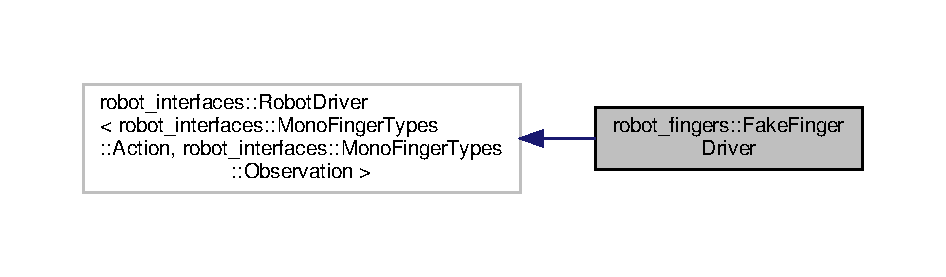
\includegraphics[width=350pt]{classrobot__fingers_1_1FakeFingerDriver__inherit__graph}
\end{center}
\end{figure}


Collaboration diagram for robot\+\_\+fingers\+:\+:Fake\+Finger\+Driver\+:
\nopagebreak
\begin{figure}[H]
\begin{center}
\leavevmode
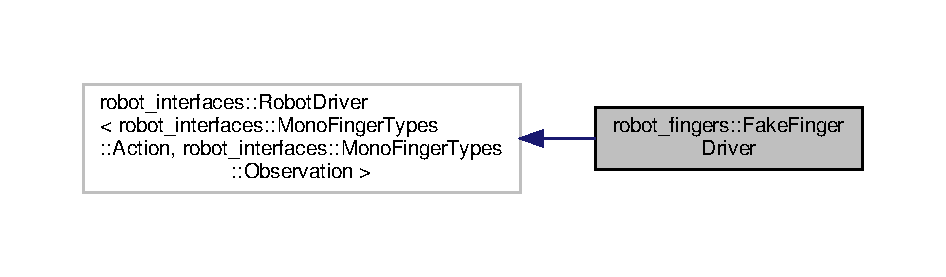
\includegraphics[width=350pt]{classrobot__fingers_1_1FakeFingerDriver__coll__graph}
\end{center}
\end{figure}
\subsection*{Public Types}
\begin{DoxyCompactItemize}
\item 
\mbox{\Hypertarget{classrobot__fingers_1_1FakeFingerDriver_a6b4051a41538c4802aa409ae09979c73}\label{classrobot__fingers_1_1FakeFingerDriver_a6b4051a41538c4802aa409ae09979c73}} 
typedef robot\+\_\+interfaces\+::\+Mono\+Finger\+Types\+::\+Action {\bfseries Action}
\item 
\mbox{\Hypertarget{classrobot__fingers_1_1FakeFingerDriver_a0d3cb596eea824a0f45179d486839a81}\label{classrobot__fingers_1_1FakeFingerDriver_a0d3cb596eea824a0f45179d486839a81}} 
typedef robot\+\_\+interfaces\+::\+Mono\+Finger\+Types\+::\+Observation {\bfseries Observation}
\item 
\mbox{\Hypertarget{classrobot__fingers_1_1FakeFingerDriver_adaad0a14dc1c21aed76746376983f0c7}\label{classrobot__fingers_1_1FakeFingerDriver_adaad0a14dc1c21aed76746376983f0c7}} 
typedef robot\+\_\+interfaces\+::\+Mono\+Finger\+Types\+::\+Action\+::\+Vector {\bfseries Vector}
\end{DoxyCompactItemize}
\subsection*{Public Member Functions}
\begin{DoxyCompactItemize}
\item 
\mbox{\Hypertarget{classrobot__fingers_1_1FakeFingerDriver_a20659a124d26cec0f1ce32c03a4d7103}\label{classrobot__fingers_1_1FakeFingerDriver_a20659a124d26cec0f1ce32c03a4d7103}} 
Observation {\bfseries get\+\_\+latest\+\_\+observation} () override
\item 
\mbox{\Hypertarget{classrobot__fingers_1_1FakeFingerDriver_a27f8b6776825a9d037a9cafad542a40f}\label{classrobot__fingers_1_1FakeFingerDriver_a27f8b6776825a9d037a9cafad542a40f}} 
Action {\bfseries apply\+\_\+action} (const Action \&desired\+\_\+action) override
\item 
\mbox{\Hypertarget{classrobot__fingers_1_1FakeFingerDriver_a490d15910b7b70c1311f4afa6d16b30a}\label{classrobot__fingers_1_1FakeFingerDriver_a490d15910b7b70c1311f4afa6d16b30a}} 
std\+::string {\bfseries get\+\_\+error} () override
\item 
\mbox{\Hypertarget{classrobot__fingers_1_1FakeFingerDriver_ad09f44f1223938439637bfc80974e033}\label{classrobot__fingers_1_1FakeFingerDriver_ad09f44f1223938439637bfc80974e033}} 
void {\bfseries shutdown} () override
\item 
\mbox{\Hypertarget{classrobot__fingers_1_1FakeFingerDriver_a1013f49d736069d57fe5fe2e2575505c}\label{classrobot__fingers_1_1FakeFingerDriver_a1013f49d736069d57fe5fe2e2575505c}} 
void {\bfseries initialize} () override
\end{DoxyCompactItemize}
\subsection*{Public Attributes}
\begin{DoxyCompactItemize}
\item 
\mbox{\Hypertarget{classrobot__fingers_1_1FakeFingerDriver_ad29266b05949f57644976262f09fedc8}\label{classrobot__fingers_1_1FakeFingerDriver_ad29266b05949f57644976262f09fedc8}} 
int {\bfseries data\+\_\+generating\+\_\+index\+\_\+} = 0
\end{DoxyCompactItemize}


The documentation for this class was generated from the following file\+:\begin{DoxyCompactItemize}
\item 
include/robot\+\_\+fingers/fake\+\_\+finger\+\_\+driver.\+hpp\end{DoxyCompactItemize}

\hypertarget{classrobot__fingers_1_1NFingerDriver}{}\section{robot\+\_\+fingers\+:\+:N\+Finger\+Driver$<$ N\+\_\+\+F\+I\+N\+G\+E\+RS $>$ Class Template Reference}
\label{classrobot__fingers_1_1NFingerDriver}\index{robot\+\_\+fingers\+::\+N\+Finger\+Driver$<$ N\+\_\+\+F\+I\+N\+G\+E\+R\+S $>$@{robot\+\_\+fingers\+::\+N\+Finger\+Driver$<$ N\+\_\+\+F\+I\+N\+G\+E\+R\+S $>$}}


Driver for the Finger robots.  




{\ttfamily \#include $<$n\+\_\+finger\+\_\+driver.\+hpp$>$}



Inheritance diagram for robot\+\_\+fingers\+:\+:N\+Finger\+Driver$<$ N\+\_\+\+F\+I\+N\+G\+E\+RS $>$\+:
\nopagebreak
\begin{figure}[H]
\begin{center}
\leavevmode
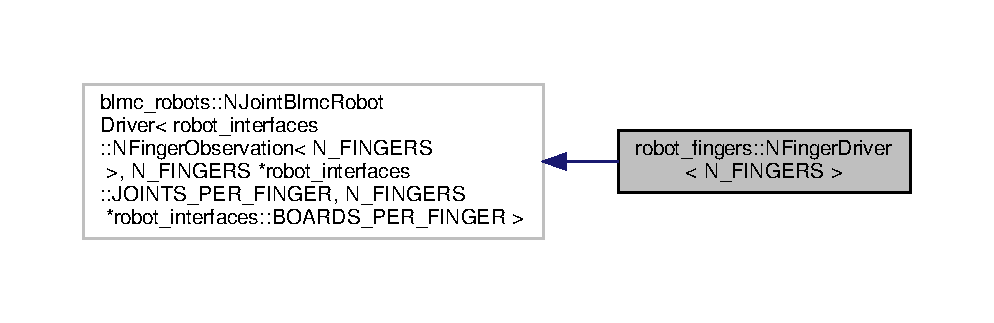
\includegraphics[width=350pt]{classrobot__fingers_1_1NFingerDriver__inherit__graph}
\end{center}
\end{figure}


Collaboration diagram for robot\+\_\+fingers\+:\+:N\+Finger\+Driver$<$ N\+\_\+\+F\+I\+N\+G\+E\+RS $>$\+:
\nopagebreak
\begin{figure}[H]
\begin{center}
\leavevmode
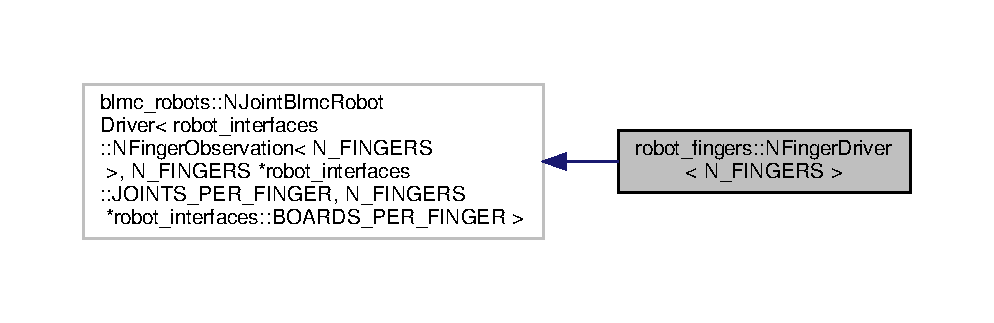
\includegraphics[width=350pt]{classrobot__fingers_1_1NFingerDriver__coll__graph}
\end{center}
\end{figure}
\subsection*{Public Types}
\begin{DoxyCompactItemize}
\item 
\mbox{\Hypertarget{classrobot__fingers_1_1NFingerDriver_a3741726de98d8380fe0e74a319142a37}\label{classrobot__fingers_1_1NFingerDriver_a3741726de98d8380fe0e74a319142a37}} 
typedef blmc\+\_\+robots\+::\+N\+Joint\+Blmc\+Robot\+Driver$<$ robot\+\_\+interfaces\+::\+N\+Finger\+Observation$<$ N\+\_\+\+F\+I\+N\+G\+E\+RS $>$, N\+\_\+\+F\+I\+N\+G\+E\+RS $\ast$robot\+\_\+interfaces\+::\+J\+O\+I\+N\+T\+S\+\_\+\+P\+E\+R\+\_\+\+F\+I\+N\+G\+ER, N\+\_\+\+F\+I\+N\+G\+E\+RS $\ast$robot\+\_\+interfaces\+::\+B\+O\+A\+R\+D\+S\+\_\+\+P\+E\+R\+\_\+\+F\+I\+N\+G\+ER $>$ {\bfseries N\+Joint\+Blmc\+Robot\+Driver}
\item 
\mbox{\Hypertarget{classrobot__fingers_1_1NFingerDriver_aeab9d2ff4949eb200742fc069439d571}\label{classrobot__fingers_1_1NFingerDriver_aeab9d2ff4949eb200742fc069439d571}} 
typedef robot\+\_\+interfaces\+::\+N\+Finger\+Observation$<$ N\+\_\+\+F\+I\+N\+G\+E\+RS $>$ {\bfseries Observation}
\end{DoxyCompactItemize}
\subsection*{Public Member Functions}
\begin{DoxyCompactItemize}
\item 
\mbox{\Hypertarget{classrobot__fingers_1_1NFingerDriver_a596ba13ac6b3f89a6078c2304c1b9700}\label{classrobot__fingers_1_1NFingerDriver_a596ba13ac6b3f89a6078c2304c1b9700}} 
Observation {\bfseries get\+\_\+latest\+\_\+observation} () override
\end{DoxyCompactItemize}


\subsection{Detailed Description}
\subsubsection*{template$<$size\+\_\+t N\+\_\+\+F\+I\+N\+G\+E\+RS$>$\newline
class robot\+\_\+fingers\+::\+N\+Finger\+Driver$<$ N\+\_\+\+F\+I\+N\+G\+E\+R\+S $>$}

Driver for the Finger robots. 

This is a generic driver for the C\+A\+N-\/based B\+L\+MC Finger Robots. It works for both a single finger and a set of multiple fingers.


\begin{DoxyTemplParams}{Template Parameters}
{\em N\+\_\+\+F\+I\+N\+G\+E\+RS} & Number of fingers on the robot. \\
\hline
\end{DoxyTemplParams}


The documentation for this class was generated from the following file\+:\begin{DoxyCompactItemize}
\item 
include/robot\+\_\+fingers/\hyperlink{n__finger__driver_8hpp}{n\+\_\+finger\+\_\+driver.\+hpp}\end{DoxyCompactItemize}

\hypertarget{classrobot__fingers_1_1OneJointDriver}{}\section{robot\+\_\+fingers\+:\+:One\+Joint\+Driver Class Reference}
\label{classrobot__fingers_1_1OneJointDriver}\index{robot\+\_\+fingers\+::\+One\+Joint\+Driver@{robot\+\_\+fingers\+::\+One\+Joint\+Driver}}


Driver for a single joint.  




{\ttfamily \#include $<$one\+\_\+joint\+\_\+driver.\+hpp$>$}



Inheritance diagram for robot\+\_\+fingers\+:\+:One\+Joint\+Driver\+:
\nopagebreak
\begin{figure}[H]
\begin{center}
\leavevmode
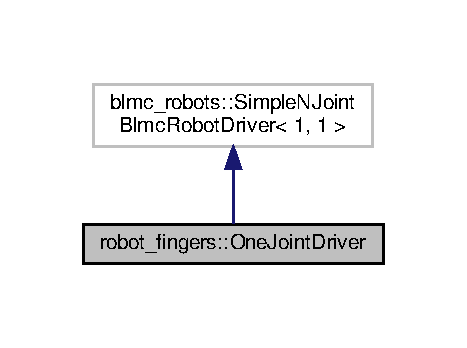
\includegraphics[width=224pt]{classrobot__fingers_1_1OneJointDriver__inherit__graph}
\end{center}
\end{figure}


Collaboration diagram for robot\+\_\+fingers\+:\+:One\+Joint\+Driver\+:
\nopagebreak
\begin{figure}[H]
\begin{center}
\leavevmode
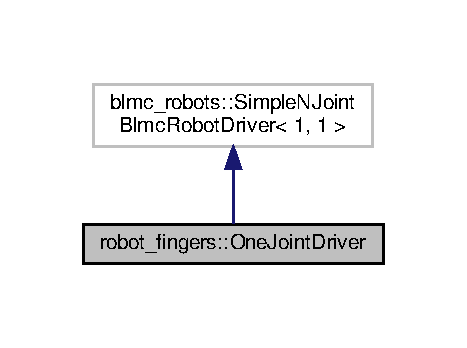
\includegraphics[width=224pt]{classrobot__fingers_1_1OneJointDriver__coll__graph}
\end{center}
\end{figure}
\subsection*{Public Member Functions}
\begin{DoxyCompactItemize}
\item 
\mbox{\Hypertarget{classrobot__fingers_1_1OneJointDriver_ac730c5dd015fa448037892967126d144}\label{classrobot__fingers_1_1OneJointDriver_ac730c5dd015fa448037892967126d144}} 
{\bfseries One\+Joint\+Driver} (const Config \&config)
\end{DoxyCompactItemize}
\subsection*{Private Member Functions}
\begin{DoxyCompactItemize}
\item 
\mbox{\Hypertarget{classrobot__fingers_1_1OneJointDriver_ad819a720c48af4020b5b88aea54e872f}\label{classrobot__fingers_1_1OneJointDriver_ad819a720c48af4020b5b88aea54e872f}} 
{\bfseries One\+Joint\+Driver} (const Motor\+Boards \&motor\+\_\+boards, const Config \&config)
\end{DoxyCompactItemize}
\subsection*{Static Private Member Functions}
\begin{DoxyCompactItemize}
\item 
\mbox{\Hypertarget{classrobot__fingers_1_1OneJointDriver_ac16ac0401586eb37920c3cccd5b5e872}\label{classrobot__fingers_1_1OneJointDriver_ac16ac0401586eb37920c3cccd5b5e872}} 
static Motors {\bfseries create\+\_\+motors} (const Motor\+Boards \&motor\+\_\+boards)
\end{DoxyCompactItemize}


\subsection{Detailed Description}
Driver for a single joint. 

Driver for a single B\+L\+MC joint. Mostly intended for testing purposes. 

The documentation for this class was generated from the following file\+:\begin{DoxyCompactItemize}
\item 
include/robot\+\_\+fingers/\hyperlink{one__joint__driver_8hpp}{one\+\_\+joint\+\_\+driver.\+hpp}\end{DoxyCompactItemize}

\hypertarget{classrobot__fingers_1_1RealFingerDriver}{}\section{robot\+\_\+fingers\+:\+:Real\+Finger\+Driver Class Reference}
\label{classrobot__fingers_1_1RealFingerDriver}\index{robot\+\_\+fingers\+::\+Real\+Finger\+Driver@{robot\+\_\+fingers\+::\+Real\+Finger\+Driver}}


Inheritance diagram for robot\+\_\+fingers\+:\+:Real\+Finger\+Driver\+:
\nopagebreak
\begin{figure}[H]
\begin{center}
\leavevmode
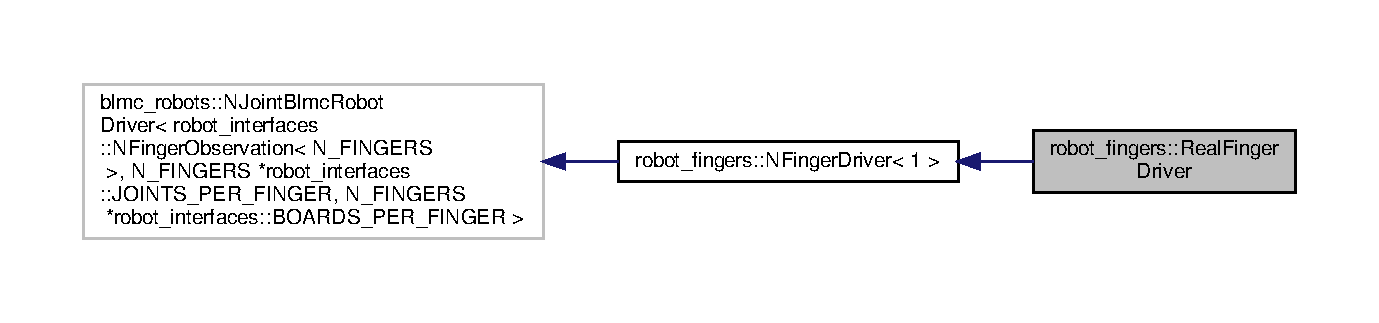
\includegraphics[width=350pt]{classrobot__fingers_1_1RealFingerDriver__inherit__graph}
\end{center}
\end{figure}


Collaboration diagram for robot\+\_\+fingers\+:\+:Real\+Finger\+Driver\+:
\nopagebreak
\begin{figure}[H]
\begin{center}
\leavevmode
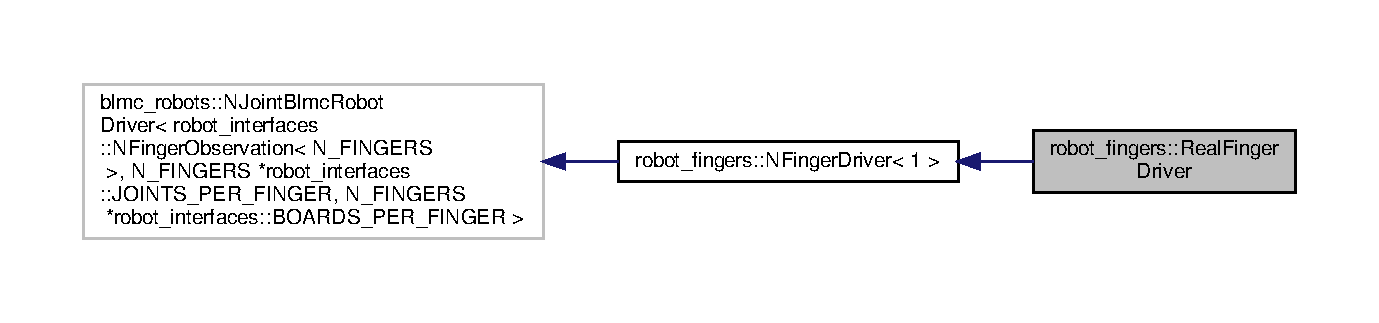
\includegraphics[width=350pt]{classrobot__fingers_1_1RealFingerDriver__coll__graph}
\end{center}
\end{figure}
\subsection*{Public Member Functions}
\begin{DoxyCompactItemize}
\item 
\mbox{\Hypertarget{classrobot__fingers_1_1RealFingerDriver_ab34c50dd9e303384802d7ee3fdaf01f3}\label{classrobot__fingers_1_1RealFingerDriver_ab34c50dd9e303384802d7ee3fdaf01f3}} 
{\bfseries Real\+Finger\+Driver} (const Config \&config)
\end{DoxyCompactItemize}
\subsection*{Private Member Functions}
\begin{DoxyCompactItemize}
\item 
\mbox{\Hypertarget{classrobot__fingers_1_1RealFingerDriver_a1e61688bf10e52d63a6497d24ad9012d}\label{classrobot__fingers_1_1RealFingerDriver_a1e61688bf10e52d63a6497d24ad9012d}} 
{\bfseries Real\+Finger\+Driver} (const Motor\+Boards \&motor\+\_\+boards, const Config \&config)
\end{DoxyCompactItemize}
\subsection*{Static Private Member Functions}
\begin{DoxyCompactItemize}
\item 
\mbox{\Hypertarget{classrobot__fingers_1_1RealFingerDriver_a5680b7497c3b3ceeba5f67346025aef1}\label{classrobot__fingers_1_1RealFingerDriver_a5680b7497c3b3ceeba5f67346025aef1}} 
static Motors {\bfseries create\+\_\+motors} (const Motor\+Boards \&motor\+\_\+boards)
\end{DoxyCompactItemize}
\subsection*{Additional Inherited Members}


The documentation for this class was generated from the following file\+:\begin{DoxyCompactItemize}
\item 
include/robot\+\_\+fingers/\hyperlink{real__finger__driver_8hpp}{real\+\_\+finger\+\_\+driver.\+hpp}\end{DoxyCompactItemize}

\hypertarget{classrobot__fingers_1_1robot_1_1Robot}{}\section{robot\+\_\+fingers.\+robot.\+Robot Class Reference}
\label{classrobot__fingers_1_1robot_1_1Robot}\index{robot\+\_\+fingers.\+robot.\+Robot@{robot\+\_\+fingers.\+robot.\+Robot}}
\subsection*{Public Member Functions}
\begin{DoxyCompactItemize}
\item 
def \hyperlink{classrobot__fingers_1_1robot_1_1Robot_ab861541dfe9f4689d9c3f842b2cd8a4e}{create\+\_\+by\+\_\+name} (cls, robot\+\_\+name)
\begin{DoxyCompactList}\small\item\em Create a {\ttfamily \hyperlink{classrobot__fingers_1_1robot_1_1Robot}{Robot}} instance for the specified robot. \end{DoxyCompactList}\item 
def \hyperlink{classrobot__fingers_1_1robot_1_1Robot_a47fe6f4f534c2e30d129f931b586590f}{\+\_\+\+\_\+init\+\_\+\+\_\+} (self, robot\+\_\+module, create\+\_\+backend\+\_\+function, config\+\_\+file\+\_\+name)
\begin{DoxyCompactList}\small\item\em Initialize the robot environment (backend and frontend). \end{DoxyCompactList}\item 
def \hyperlink{classrobot__fingers_1_1robot_1_1Robot_a68fd76fde66f13b697e2492932b2dca5}{initialize} (self)
\begin{DoxyCompactList}\small\item\em Initialize the robot. \end{DoxyCompactList}\end{DoxyCompactItemize}
\subsection*{Static Public Member Functions}
\begin{DoxyCompactItemize}
\item 
def \hyperlink{classrobot__fingers_1_1robot_1_1Robot_ae4d1f723105c1d3c00c49db2e7c283ae}{get\+\_\+supported\+\_\+robots} ()
\begin{DoxyCompactList}\small\item\em Get list of robots supported by {\ttfamily create\+\_\+by\+\_\+name}. \end{DoxyCompactList}\end{DoxyCompactItemize}
\subsection*{Public Attributes}
\begin{DoxyCompactItemize}
\item 
\mbox{\Hypertarget{classrobot__fingers_1_1robot_1_1Robot_a2a0232b3acf259eeddb318d312887815}\label{classrobot__fingers_1_1robot_1_1Robot_a2a0232b3acf259eeddb318d312887815}} 
{\bfseries Action}
\item 
\mbox{\Hypertarget{classrobot__fingers_1_1robot_1_1Robot_a727813d76f35690ee282446d082c943e}\label{classrobot__fingers_1_1robot_1_1Robot_a727813d76f35690ee282446d082c943e}} 
{\bfseries robot\+\_\+data}
\item 
\mbox{\Hypertarget{classrobot__fingers_1_1robot_1_1Robot_a0ae4a629cc745c551fe6941eeeb19523}\label{classrobot__fingers_1_1robot_1_1Robot_a0ae4a629cc745c551fe6941eeeb19523}} 
{\bfseries backend}
\item 
\mbox{\Hypertarget{classrobot__fingers_1_1robot_1_1Robot_ac538343aab9e49a97c202da1cee4e030}\label{classrobot__fingers_1_1robot_1_1Robot_ac538343aab9e49a97c202da1cee4e030}} 
{\bfseries frontend}
\item 
\mbox{\Hypertarget{classrobot__fingers_1_1robot_1_1Robot_ac0479c96ecf5a2ef5d9e836bb0a1a463}\label{classrobot__fingers_1_1robot_1_1Robot_ac0479c96ecf5a2ef5d9e836bb0a1a463}} 
{\bfseries logger}
\end{DoxyCompactItemize}


\subsection{Constructor \& Destructor Documentation}
\mbox{\Hypertarget{classrobot__fingers_1_1robot_1_1Robot_a47fe6f4f534c2e30d129f931b586590f}\label{classrobot__fingers_1_1robot_1_1Robot_a47fe6f4f534c2e30d129f931b586590f}} 
\index{robot\+\_\+fingers\+::robot\+::\+Robot@{robot\+\_\+fingers\+::robot\+::\+Robot}!\+\_\+\+\_\+init\+\_\+\+\_\+@{\+\_\+\+\_\+init\+\_\+\+\_\+}}
\index{\+\_\+\+\_\+init\+\_\+\+\_\+@{\+\_\+\+\_\+init\+\_\+\+\_\+}!robot\+\_\+fingers\+::robot\+::\+Robot@{robot\+\_\+fingers\+::robot\+::\+Robot}}
\subsubsection{\texorpdfstring{\+\_\+\+\_\+init\+\_\+\+\_\+()}{\_\_init\_\_()}}
{\footnotesize\ttfamily def robot\+\_\+fingers.\+robot.\+Robot.\+\_\+\+\_\+init\+\_\+\+\_\+ (\begin{DoxyParamCaption}\item[{}]{self,  }\item[{}]{robot\+\_\+module,  }\item[{}]{create\+\_\+backend\+\_\+function,  }\item[{}]{config\+\_\+file\+\_\+name }\end{DoxyParamCaption})}



Initialize the robot environment (backend and frontend). 

\+:param robot\+\_\+module\+: The module that defines the robot classes (i.\+e. {\ttfamily Data}, {\ttfamily Frontend}, {\ttfamily Backend}, ...) \+:param create\+\_\+backend\+\_\+function\+: Function to create the robot backend. \+:param config\+\_\+file\+\_\+name\+: Either an absolute path to a config file (needs to start with \char`\"{}/\char`\"{} in this case) or the name of a config file located in robot\+\_\+fingers/config. 

\subsection{Member Function Documentation}
\mbox{\Hypertarget{classrobot__fingers_1_1robot_1_1Robot_ab861541dfe9f4689d9c3f842b2cd8a4e}\label{classrobot__fingers_1_1robot_1_1Robot_ab861541dfe9f4689d9c3f842b2cd8a4e}} 
\index{robot\+\_\+fingers\+::robot\+::\+Robot@{robot\+\_\+fingers\+::robot\+::\+Robot}!create\+\_\+by\+\_\+name@{create\+\_\+by\+\_\+name}}
\index{create\+\_\+by\+\_\+name@{create\+\_\+by\+\_\+name}!robot\+\_\+fingers\+::robot\+::\+Robot@{robot\+\_\+fingers\+::robot\+::\+Robot}}
\subsubsection{\texorpdfstring{create\+\_\+by\+\_\+name()}{create\_by\_name()}}
{\footnotesize\ttfamily def robot\+\_\+fingers.\+robot.\+Robot.\+create\+\_\+by\+\_\+name (\begin{DoxyParamCaption}\item[{}]{cls,  }\item[{}]{robot\+\_\+name }\end{DoxyParamCaption})}



Create a {\ttfamily \hyperlink{classrobot__fingers_1_1robot_1_1Robot}{Robot}} instance for the specified robot. 


\begin{DoxyParams}{Parameters}
{\em robot\+\_\+name} & Name of the robots. See \+:meth\+:{\ttfamily \hyperlink{classrobot__fingers_1_1robot_1_1Robot_ae4d1f723105c1d3c00c49db2e7c283ae}{Robot.\+get\+\_\+supported\+\_\+robots}} for a list of supported robots.\\
\hline
\end{DoxyParams}
\begin{DoxyReturn}{Returns}


\hyperlink{classrobot__fingers_1_1robot_1_1Robot}{Robot} A {\ttfamily \hyperlink{classrobot__fingers_1_1robot_1_1Robot}{Robot}} instance for the specified robot. 
\end{DoxyReturn}
\mbox{\Hypertarget{classrobot__fingers_1_1robot_1_1Robot_ae4d1f723105c1d3c00c49db2e7c283ae}\label{classrobot__fingers_1_1robot_1_1Robot_ae4d1f723105c1d3c00c49db2e7c283ae}} 
\index{robot\+\_\+fingers\+::robot\+::\+Robot@{robot\+\_\+fingers\+::robot\+::\+Robot}!get\+\_\+supported\+\_\+robots@{get\+\_\+supported\+\_\+robots}}
\index{get\+\_\+supported\+\_\+robots@{get\+\_\+supported\+\_\+robots}!robot\+\_\+fingers\+::robot\+::\+Robot@{robot\+\_\+fingers\+::robot\+::\+Robot}}
\subsubsection{\texorpdfstring{get\+\_\+supported\+\_\+robots()}{get\_supported\_robots()}}
{\footnotesize\ttfamily def robot\+\_\+fingers.\+robot.\+Robot.\+get\+\_\+supported\+\_\+robots (\begin{DoxyParamCaption}{ }\end{DoxyParamCaption})\hspace{0.3cm}{\ttfamily [static]}}



Get list of robots supported by {\ttfamily create\+\_\+by\+\_\+name}. 

\begin{DoxyReturn}{Returns}
List of supported robot names. 
\end{DoxyReturn}
\mbox{\Hypertarget{classrobot__fingers_1_1robot_1_1Robot_a68fd76fde66f13b697e2492932b2dca5}\label{classrobot__fingers_1_1robot_1_1Robot_a68fd76fde66f13b697e2492932b2dca5}} 
\index{robot\+\_\+fingers\+::robot\+::\+Robot@{robot\+\_\+fingers\+::robot\+::\+Robot}!initialize@{initialize}}
\index{initialize@{initialize}!robot\+\_\+fingers\+::robot\+::\+Robot@{robot\+\_\+fingers\+::robot\+::\+Robot}}
\subsubsection{\texorpdfstring{initialize()}{initialize()}}
{\footnotesize\ttfamily def robot\+\_\+fingers.\+robot.\+Robot.\+initialize (\begin{DoxyParamCaption}\item[{}]{self }\end{DoxyParamCaption})}



Initialize the robot. 



The documentation for this class was generated from the following file\+:\begin{DoxyCompactItemize}
\item 
python/robot\+\_\+fingers/robot.\+py\end{DoxyCompactItemize}

\hypertarget{classdemonstrate__trajectory_1_1SimpleCursesGUI}{}\section{demonstrate\+\_\+trajectory.\+Simple\+Curses\+G\+UI Class Reference}
\label{classdemonstrate__trajectory_1_1SimpleCursesGUI}\index{demonstrate\+\_\+trajectory.\+Simple\+Curses\+G\+UI@{demonstrate\+\_\+trajectory.\+Simple\+Curses\+G\+UI}}


Wrapper around curses to manage simple generic G\+U\+Is.  


\subsection*{Public Member Functions}
\begin{DoxyCompactItemize}
\item 
def \hyperlink{classdemonstrate__trajectory_1_1SimpleCursesGUI_a75bb22b79a52c4aaaf98c5349b2d5992}{\+\_\+\+\_\+init\+\_\+\+\_\+} (self, win, title, status\+\_\+line=None)
\begin{DoxyCompactList}\small\item\em Initialize. \end{DoxyCompactList}\item 
def \hyperlink{classdemonstrate__trajectory_1_1SimpleCursesGUI_abda27a311898db3c5b5f6dc9ad4351bf}{display\+\_\+error} (self, message)
\begin{DoxyCompactList}\small\item\em Display error message and wait until user presses a key. \end{DoxyCompactList}\item 
def \hyperlink{classdemonstrate__trajectory_1_1SimpleCursesGUI_ae9ba316b4409ee4a52db5f373b833948}{update\+\_\+screen} (self, lines)
\begin{DoxyCompactList}\small\item\em Update the screen with the given lines of text. \end{DoxyCompactList}\item 
def \hyperlink{classdemonstrate__trajectory_1_1SimpleCursesGUI_a273895ec6e0192cc5284af7f91023c68}{get\+\_\+pressed\+\_\+key} (self)
\begin{DoxyCompactList}\small\item\em Get key pressed by the user. \end{DoxyCompactList}\end{DoxyCompactItemize}
\subsection*{Public Attributes}
\begin{DoxyCompactItemize}
\item 
\mbox{\Hypertarget{classdemonstrate__trajectory_1_1SimpleCursesGUI_ae25361dcf2c4119e655cf0b1cfaf1415}\label{classdemonstrate__trajectory_1_1SimpleCursesGUI_ae25361dcf2c4119e655cf0b1cfaf1415}} 
{\bfseries win}
\item 
\mbox{\Hypertarget{classdemonstrate__trajectory_1_1SimpleCursesGUI_a4e078b6f93564072c262880278db6291}\label{classdemonstrate__trajectory_1_1SimpleCursesGUI_a4e078b6f93564072c262880278db6291}} 
{\bfseries title}
\item 
\mbox{\Hypertarget{classdemonstrate__trajectory_1_1SimpleCursesGUI_a1fd2de53b6b7aa388b127071707e4d57}\label{classdemonstrate__trajectory_1_1SimpleCursesGUI_a1fd2de53b6b7aa388b127071707e4d57}} 
{\bfseries status\+\_\+line}
\end{DoxyCompactItemize}


\subsection{Detailed Description}
Wrapper around curses to manage simple generic G\+U\+Is. 

A very simple curses interface with a title at the top, a static status line at the bottom and some arbitrary text in between that can be updated. 

\subsection{Constructor \& Destructor Documentation}
\mbox{\Hypertarget{classdemonstrate__trajectory_1_1SimpleCursesGUI_a75bb22b79a52c4aaaf98c5349b2d5992}\label{classdemonstrate__trajectory_1_1SimpleCursesGUI_a75bb22b79a52c4aaaf98c5349b2d5992}} 
\index{demonstrate\+\_\+trajectory\+::\+Simple\+Curses\+G\+UI@{demonstrate\+\_\+trajectory\+::\+Simple\+Curses\+G\+UI}!\+\_\+\+\_\+init\+\_\+\+\_\+@{\+\_\+\+\_\+init\+\_\+\+\_\+}}
\index{\+\_\+\+\_\+init\+\_\+\+\_\+@{\+\_\+\+\_\+init\+\_\+\+\_\+}!demonstrate\+\_\+trajectory\+::\+Simple\+Curses\+G\+UI@{demonstrate\+\_\+trajectory\+::\+Simple\+Curses\+G\+UI}}
\subsubsection{\texorpdfstring{\+\_\+\+\_\+init\+\_\+\+\_\+()}{\_\_init\_\_()}}
{\footnotesize\ttfamily def demonstrate\+\_\+trajectory.\+Simple\+Curses\+G\+U\+I.\+\_\+\+\_\+init\+\_\+\+\_\+ (\begin{DoxyParamCaption}\item[{}]{self,  }\item[{}]{win,  }\item[{}]{title,  }\item[{}]{status\+\_\+line = {\ttfamily None} }\end{DoxyParamCaption})}



Initialize. 


\begin{DoxyParams}{Parameters}
{\em win} & Curses window. \\
\hline
\end{DoxyParams}


\subsection{Member Function Documentation}
\mbox{\Hypertarget{classdemonstrate__trajectory_1_1SimpleCursesGUI_abda27a311898db3c5b5f6dc9ad4351bf}\label{classdemonstrate__trajectory_1_1SimpleCursesGUI_abda27a311898db3c5b5f6dc9ad4351bf}} 
\index{demonstrate\+\_\+trajectory\+::\+Simple\+Curses\+G\+UI@{demonstrate\+\_\+trajectory\+::\+Simple\+Curses\+G\+UI}!display\+\_\+error@{display\+\_\+error}}
\index{display\+\_\+error@{display\+\_\+error}!demonstrate\+\_\+trajectory\+::\+Simple\+Curses\+G\+UI@{demonstrate\+\_\+trajectory\+::\+Simple\+Curses\+G\+UI}}
\subsubsection{\texorpdfstring{display\+\_\+error()}{display\_error()}}
{\footnotesize\ttfamily def demonstrate\+\_\+trajectory.\+Simple\+Curses\+G\+U\+I.\+display\+\_\+error (\begin{DoxyParamCaption}\item[{}]{self,  }\item[{}]{message }\end{DoxyParamCaption})}



Display error message and wait until user presses a key. 


\begin{DoxyParams}{Parameters}
{\em message} & The error message that is displayed. \\
\hline
\end{DoxyParams}
\mbox{\Hypertarget{classdemonstrate__trajectory_1_1SimpleCursesGUI_a273895ec6e0192cc5284af7f91023c68}\label{classdemonstrate__trajectory_1_1SimpleCursesGUI_a273895ec6e0192cc5284af7f91023c68}} 
\index{demonstrate\+\_\+trajectory\+::\+Simple\+Curses\+G\+UI@{demonstrate\+\_\+trajectory\+::\+Simple\+Curses\+G\+UI}!get\+\_\+pressed\+\_\+key@{get\+\_\+pressed\+\_\+key}}
\index{get\+\_\+pressed\+\_\+key@{get\+\_\+pressed\+\_\+key}!demonstrate\+\_\+trajectory\+::\+Simple\+Curses\+G\+UI@{demonstrate\+\_\+trajectory\+::\+Simple\+Curses\+G\+UI}}
\subsubsection{\texorpdfstring{get\+\_\+pressed\+\_\+key()}{get\_pressed\_key()}}
{\footnotesize\ttfamily def demonstrate\+\_\+trajectory.\+Simple\+Curses\+G\+U\+I.\+get\+\_\+pressed\+\_\+key (\begin{DoxyParamCaption}\item[{}]{self }\end{DoxyParamCaption})}



Get key pressed by the user. 

\mbox{\Hypertarget{classdemonstrate__trajectory_1_1SimpleCursesGUI_ae9ba316b4409ee4a52db5f373b833948}\label{classdemonstrate__trajectory_1_1SimpleCursesGUI_ae9ba316b4409ee4a52db5f373b833948}} 
\index{demonstrate\+\_\+trajectory\+::\+Simple\+Curses\+G\+UI@{demonstrate\+\_\+trajectory\+::\+Simple\+Curses\+G\+UI}!update\+\_\+screen@{update\+\_\+screen}}
\index{update\+\_\+screen@{update\+\_\+screen}!demonstrate\+\_\+trajectory\+::\+Simple\+Curses\+G\+UI@{demonstrate\+\_\+trajectory\+::\+Simple\+Curses\+G\+UI}}
\subsubsection{\texorpdfstring{update\+\_\+screen()}{update\_screen()}}
{\footnotesize\ttfamily def demonstrate\+\_\+trajectory.\+Simple\+Curses\+G\+U\+I.\+update\+\_\+screen (\begin{DoxyParamCaption}\item[{}]{self,  }\item[{}]{lines }\end{DoxyParamCaption})}



Update the screen with the given lines of text. 


\begin{DoxyParams}{Parameters}
{\em lines} & List of strings. They are drawn in separate lines. \\
\hline
\end{DoxyParams}


The documentation for this class was generated from the following file\+:\begin{DoxyCompactItemize}
\item 
scripts/demonstrate\+\_\+trajectory.\+py\end{DoxyCompactItemize}

\hypertarget{classrobot__fingers_1_1TriFingerDriver}{}\section{robot\+\_\+fingers\+:\+:Tri\+Finger\+Driver Class Reference}
\label{classrobot__fingers_1_1TriFingerDriver}\index{robot\+\_\+fingers\+::\+Tri\+Finger\+Driver@{robot\+\_\+fingers\+::\+Tri\+Finger\+Driver}}


Inheritance diagram for robot\+\_\+fingers\+:\+:Tri\+Finger\+Driver\+:
\nopagebreak
\begin{figure}[H]
\begin{center}
\leavevmode
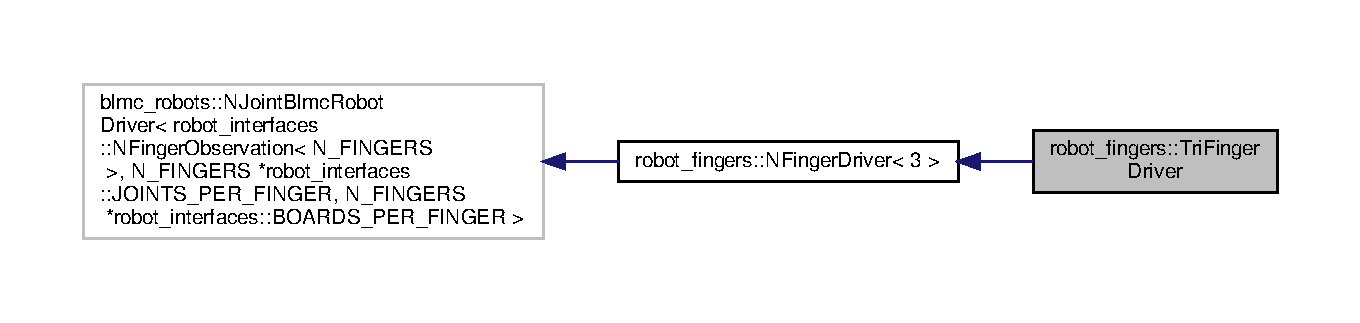
\includegraphics[width=350pt]{classrobot__fingers_1_1TriFingerDriver__inherit__graph}
\end{center}
\end{figure}


Collaboration diagram for robot\+\_\+fingers\+:\+:Tri\+Finger\+Driver\+:
\nopagebreak
\begin{figure}[H]
\begin{center}
\leavevmode
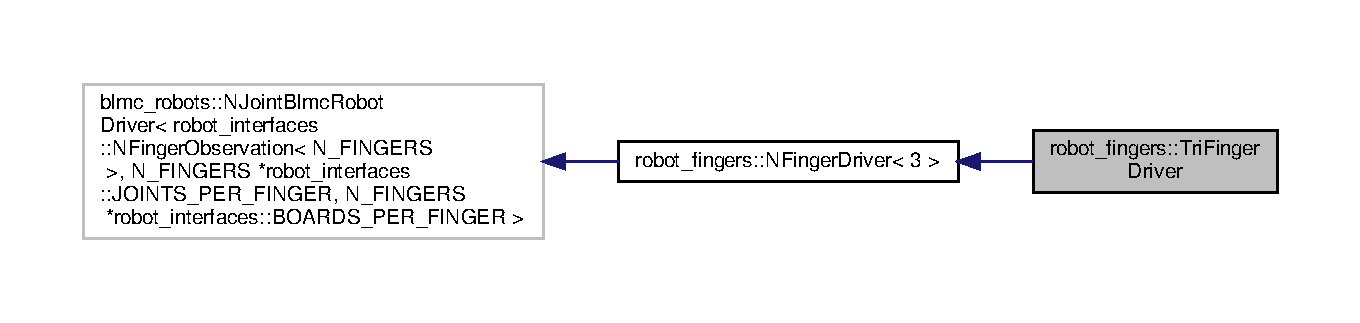
\includegraphics[width=350pt]{classrobot__fingers_1_1TriFingerDriver__coll__graph}
\end{center}
\end{figure}
\subsection*{Public Member Functions}
\begin{DoxyCompactItemize}
\item 
\mbox{\Hypertarget{classrobot__fingers_1_1TriFingerDriver_a6fa7ba8449fcf922f7d87fea296c9eca}\label{classrobot__fingers_1_1TriFingerDriver_a6fa7ba8449fcf922f7d87fea296c9eca}} 
{\bfseries Tri\+Finger\+Driver} (const Config \&config)
\end{DoxyCompactItemize}
\subsection*{Private Member Functions}
\begin{DoxyCompactItemize}
\item 
\mbox{\Hypertarget{classrobot__fingers_1_1TriFingerDriver_aa476efb16c779276941ff1ba6da6c28a}\label{classrobot__fingers_1_1TriFingerDriver_aa476efb16c779276941ff1ba6da6c28a}} 
{\bfseries Tri\+Finger\+Driver} (const Motor\+Boards \&motor\+\_\+boards, const Config \&config)
\end{DoxyCompactItemize}
\subsection*{Static Private Member Functions}
\begin{DoxyCompactItemize}
\item 
\mbox{\Hypertarget{classrobot__fingers_1_1TriFingerDriver_aadad79c20c522db342cb13ea9d7f53fa}\label{classrobot__fingers_1_1TriFingerDriver_aadad79c20c522db342cb13ea9d7f53fa}} 
static Motors {\bfseries create\+\_\+motors} (const Motor\+Boards \&motor\+\_\+boards)
\end{DoxyCompactItemize}
\subsection*{Additional Inherited Members}


The documentation for this class was generated from the following file\+:\begin{DoxyCompactItemize}
\item 
include/robot\+\_\+fingers/\hyperlink{trifinger__driver_8hpp}{trifinger\+\_\+driver.\+hpp}\end{DoxyCompactItemize}

\hypertarget{classrobot__fingers_1_1TriFingerPlatformFrontend}{}\section{robot\+\_\+fingers\+:\+:Tri\+Finger\+Platform\+Frontend Class Reference}
\label{classrobot__fingers_1_1TriFingerPlatformFrontend}\index{robot\+\_\+fingers\+::\+Tri\+Finger\+Platform\+Frontend@{robot\+\_\+fingers\+::\+Tri\+Finger\+Platform\+Frontend}}


Combined frontend for the Tri\+Finger Platform.  




{\ttfamily \#include $<$trifinger\+\_\+platform\+\_\+frontend.\+hpp$>$}

\subsection*{Public Types}
\begin{DoxyCompactItemize}
\item 
\mbox{\Hypertarget{classrobot__fingers_1_1TriFingerPlatformFrontend_af657fd0a6ea4023926ab23a225ca3bab}\label{classrobot__fingers_1_1TriFingerPlatformFrontend_af657fd0a6ea4023926ab23a225ca3bab}} 
typedef robot\+\_\+interfaces\+::\+Tri\+Finger\+Types\+::\+Action {\bfseries Action}
\item 
\mbox{\Hypertarget{classrobot__fingers_1_1TriFingerPlatformFrontend_a993606d1334ac3d932ba9b9637388cab}\label{classrobot__fingers_1_1TriFingerPlatformFrontend_a993606d1334ac3d932ba9b9637388cab}} 
typedef robot\+\_\+interfaces\+::\+Tri\+Finger\+Types\+::\+Observation {\bfseries Robot\+Observation}
\item 
\mbox{\Hypertarget{classrobot__fingers_1_1TriFingerPlatformFrontend_a2bb400ff94b8c528fd3be4a3112bda81}\label{classrobot__fingers_1_1TriFingerPlatformFrontend_a2bb400ff94b8c528fd3be4a3112bda81}} 
typedef robot\+\_\+interfaces\+::\+Status {\bfseries Robot\+Status}
\item 
\mbox{\Hypertarget{classrobot__fingers_1_1TriFingerPlatformFrontend_a96f578b30c6f8e2220a8cbccc91974c1}\label{classrobot__fingers_1_1TriFingerPlatformFrontend_a96f578b30c6f8e2220a8cbccc91974c1}} 
typedef trifinger\+\_\+cameras\+::\+Tri\+Camera\+Observation {\bfseries Camera\+Observation}
\end{DoxyCompactItemize}
\subsection*{Public Member Functions}
\begin{DoxyCompactItemize}
\item 
\hyperlink{classrobot__fingers_1_1TriFingerPlatformFrontend_a47150cf36520116808333d5c3e8a2fdc}{Tri\+Finger\+Platform\+Frontend} (robot\+\_\+interfaces\+::\+Tri\+Finger\+Types\+::\+Base\+Data\+Ptr robot\+\_\+data, trifinger\+\_\+object\+\_\+tracking\+::\+Object\+Tracker\+Data\+::\+Ptr object\+\_\+tracker\+\_\+data, std\+::shared\+\_\+ptr$<$ robot\+\_\+interfaces\+::\+Sensor\+Data$<$ Camera\+Observation $>$$>$ camera\+\_\+data)
\begin{DoxyCompactList}\small\item\em Initialize with data instances for all internal frontends. \end{DoxyCompactList}\item 
\hyperlink{classrobot__fingers_1_1TriFingerPlatformFrontend_aea53f5c5b5443f9b481b33392b5caa25}{Tri\+Finger\+Platform\+Frontend} ()
\begin{DoxyCompactList}\small\item\em Initialize with default data instances. \end{DoxyCompactList}\item 
time\+\_\+series\+::\+Index \hyperlink{classrobot__fingers_1_1TriFingerPlatformFrontend_a474d2d6fd6c48fc16ccd60ac2bc21c2f}{append\+\_\+desired\+\_\+action} (const Action \&desired\+\_\+action)
\begin{DoxyCompactList}\small\item\em Append a desired robot action to the action queue. \end{DoxyCompactList}\item 
Robot\+Observation \hyperlink{classrobot__fingers_1_1TriFingerPlatformFrontend_a86149ce45a4ddada714eb0e0fde20e66}{get\+\_\+robot\+\_\+observation} (const time\+\_\+series\+::\+Index \&t) const
\begin{DoxyCompactList}\small\item\em Get robot observation of the time step t. \end{DoxyCompactList}\item 
Action \hyperlink{classrobot__fingers_1_1TriFingerPlatformFrontend_acdb76e148024bfdcb59bf06a92f30222}{get\+\_\+desired\+\_\+action} (const time\+\_\+series\+::\+Index \&t) const
\begin{DoxyCompactList}\small\item\em Get desired action of time step t. \end{DoxyCompactList}\item 
Action \hyperlink{classrobot__fingers_1_1TriFingerPlatformFrontend_a7c0d56e7e1096a3ab299a45e8b832d54}{get\+\_\+applied\+\_\+action} (const time\+\_\+series\+::\+Index \&t) const
\begin{DoxyCompactList}\small\item\em Get actually applied action of time step t. \end{DoxyCompactList}\item 
Robot\+Status \hyperlink{classrobot__fingers_1_1TriFingerPlatformFrontend_afc30cd1aecd9967045a0365c21f964fe}{get\+\_\+robot\+\_\+status} (const time\+\_\+series\+::\+Index \&t) const
\begin{DoxyCompactList}\small\item\em Get robot status of time step t. \end{DoxyCompactList}\item 
time\+\_\+series\+::\+Timestamp \hyperlink{classrobot__fingers_1_1TriFingerPlatformFrontend_abf6ed97b5f5711058030733fb283aad6}{get\+\_\+timestamp\+\_\+ms} (const time\+\_\+series\+::\+Index \&t) const
\begin{DoxyCompactList}\small\item\em Get timestamp (in milliseconds) of time step t. \end{DoxyCompactList}\item 
time\+\_\+series\+::\+Index \hyperlink{classrobot__fingers_1_1TriFingerPlatformFrontend_a9c97379d70b40a023609521a83253177}{get\+\_\+current\+\_\+timeindex} () const
\begin{DoxyCompactList}\small\item\em Get the current time index. \end{DoxyCompactList}\item 
void \hyperlink{classrobot__fingers_1_1TriFingerPlatformFrontend_a0dc8d9e0d6e26053194e223ac29fc8c4}{wait\+\_\+until\+\_\+timeindex} (const time\+\_\+series\+::\+Index \&t) const
\begin{DoxyCompactList}\small\item\em Wait until time step t. \end{DoxyCompactList}\item 
trifinger\+\_\+object\+\_\+tracking\+::\+Object\+Pose \hyperlink{classrobot__fingers_1_1TriFingerPlatformFrontend_abb39cc97fbf08af6942f2de3e99e6f54}{get\+\_\+object\+\_\+pose} (const time\+\_\+series\+::\+Index t) const
\begin{DoxyCompactList}\small\item\em Get observation of the object tracker of time step t. \end{DoxyCompactList}\item 
Camera\+Observation \hyperlink{classrobot__fingers_1_1TriFingerPlatformFrontend_a2b83c7b23977185f4a522e16077b204a}{get\+\_\+camera\+\_\+observation} (const time\+\_\+series\+::\+Index t) const
\begin{DoxyCompactList}\small\item\em Get camera images of time step t. \end{DoxyCompactList}\end{DoxyCompactItemize}
\subsection*{Private Member Functions}
\begin{DoxyCompactItemize}
\item 
{\footnotesize template$<$typename Frontend\+Type $>$ }\\time\+\_\+series\+::\+Index \hyperlink{classrobot__fingers_1_1TriFingerPlatformFrontend_a4c67fd3d8d1e887ed0f5b1b8ec2d30b3}{find\+\_\+matching\+\_\+timeindex} (const Frontend\+Type \&other\+\_\+frontend, const time\+\_\+series\+::\+Index t\+\_\+robot) const
\begin{DoxyCompactList}\small\item\em Find time index of frontend that matches with the given robot time index. \end{DoxyCompactList}\end{DoxyCompactItemize}
\subsection*{Private Attributes}
\begin{DoxyCompactItemize}
\item 
\mbox{\Hypertarget{classrobot__fingers_1_1TriFingerPlatformFrontend_aa8cef15571ffada758d86370b86b8777}\label{classrobot__fingers_1_1TriFingerPlatformFrontend_aa8cef15571ffada758d86370b86b8777}} 
robot\+\_\+interfaces\+::\+Tri\+Finger\+Types\+::\+Frontend {\bfseries robot\+\_\+frontend\+\_\+}
\item 
\mbox{\Hypertarget{classrobot__fingers_1_1TriFingerPlatformFrontend_a7475483ecc42aba5910e7b3bceeecde3}\label{classrobot__fingers_1_1TriFingerPlatformFrontend_a7475483ecc42aba5910e7b3bceeecde3}} 
trifinger\+\_\+object\+\_\+tracking\+::\+Object\+Tracker\+Frontend {\bfseries object\+\_\+tracker\+\_\+frontend\+\_\+}
\item 
\mbox{\Hypertarget{classrobot__fingers_1_1TriFingerPlatformFrontend_a075fa9bb1d76bbb47955e2ce6126a0e9}\label{classrobot__fingers_1_1TriFingerPlatformFrontend_a075fa9bb1d76bbb47955e2ce6126a0e9}} 
robot\+\_\+interfaces\+::\+Sensor\+Frontend$<$ Camera\+Observation $>$ {\bfseries camera\+\_\+frontend\+\_\+}
\end{DoxyCompactItemize}


\subsection{Detailed Description}
Combined frontend for the Tri\+Finger Platform. 

This class combines the frontends for robot, cameras and object tracking in one class using unified time indices.

Internally the different frontends all have their own time indices which are unrelated to each other. In this combined class, the time index used is the one that belongs to the robot frontend. When accessing observations of the other frontends, it also takes this index t and internally matches it to the time index t\+\_\+o that was active in the other frontend at the time of t.

\begin{DoxyRefDesc}{Todo}
\item[\hyperlink{todo__todo000001}{Todo}]Methods to get timestamp from camera or object tracker? \end{DoxyRefDesc}


\subsection{Constructor \& Destructor Documentation}
\mbox{\Hypertarget{classrobot__fingers_1_1TriFingerPlatformFrontend_a47150cf36520116808333d5c3e8a2fdc}\label{classrobot__fingers_1_1TriFingerPlatformFrontend_a47150cf36520116808333d5c3e8a2fdc}} 
\index{robot\+\_\+fingers\+::\+Tri\+Finger\+Platform\+Frontend@{robot\+\_\+fingers\+::\+Tri\+Finger\+Platform\+Frontend}!Tri\+Finger\+Platform\+Frontend@{Tri\+Finger\+Platform\+Frontend}}
\index{Tri\+Finger\+Platform\+Frontend@{Tri\+Finger\+Platform\+Frontend}!robot\+\_\+fingers\+::\+Tri\+Finger\+Platform\+Frontend@{robot\+\_\+fingers\+::\+Tri\+Finger\+Platform\+Frontend}}
\subsubsection{\texorpdfstring{Tri\+Finger\+Platform\+Frontend()}{TriFingerPlatformFrontend()}\hspace{0.1cm}{\footnotesize\ttfamily [1/2]}}
{\footnotesize\ttfamily robot\+\_\+fingers\+::\+Tri\+Finger\+Platform\+Frontend\+::\+Tri\+Finger\+Platform\+Frontend (\begin{DoxyParamCaption}\item[{robot\+\_\+interfaces\+::\+Tri\+Finger\+Types\+::\+Base\+Data\+Ptr}]{robot\+\_\+data,  }\item[{trifinger\+\_\+object\+\_\+tracking\+::\+Object\+Tracker\+Data\+::\+Ptr}]{object\+\_\+tracker\+\_\+data,  }\item[{std\+::shared\+\_\+ptr$<$ robot\+\_\+interfaces\+::\+Sensor\+Data$<$ Camera\+Observation $>$$>$}]{camera\+\_\+data }\end{DoxyParamCaption})}



Initialize with data instances for all internal frontends. 


\begin{DoxyParams}{Parameters}
{\em robot\+\_\+data} & Robot\+Data instance used by the robot frontend. \\
\hline
{\em object\+\_\+tracker\+\_\+data} & Object\+Tracker\+Data instance used by the object tracker frontend. \\
\hline
{\em camera\+\_\+data} & Sensor\+Data instance, used by the camera frontend. \\
\hline
\end{DoxyParams}
\mbox{\Hypertarget{classrobot__fingers_1_1TriFingerPlatformFrontend_aea53f5c5b5443f9b481b33392b5caa25}\label{classrobot__fingers_1_1TriFingerPlatformFrontend_aea53f5c5b5443f9b481b33392b5caa25}} 
\index{robot\+\_\+fingers\+::\+Tri\+Finger\+Platform\+Frontend@{robot\+\_\+fingers\+::\+Tri\+Finger\+Platform\+Frontend}!Tri\+Finger\+Platform\+Frontend@{Tri\+Finger\+Platform\+Frontend}}
\index{Tri\+Finger\+Platform\+Frontend@{Tri\+Finger\+Platform\+Frontend}!robot\+\_\+fingers\+::\+Tri\+Finger\+Platform\+Frontend@{robot\+\_\+fingers\+::\+Tri\+Finger\+Platform\+Frontend}}
\subsubsection{\texorpdfstring{Tri\+Finger\+Platform\+Frontend()}{TriFingerPlatformFrontend()}\hspace{0.1cm}{\footnotesize\ttfamily [2/2]}}
{\footnotesize\ttfamily robot\+\_\+fingers\+::\+Tri\+Finger\+Platform\+Frontend\+::\+Tri\+Finger\+Platform\+Frontend (\begin{DoxyParamCaption}{ }\end{DoxyParamCaption})}



Initialize with default data instances. 

Creates for each internal frontend a corresponding mutli-\/process data instance with the default shared memory ID for the corresponding data type. 

\subsection{Member Function Documentation}
\mbox{\Hypertarget{classrobot__fingers_1_1TriFingerPlatformFrontend_a474d2d6fd6c48fc16ccd60ac2bc21c2f}\label{classrobot__fingers_1_1TriFingerPlatformFrontend_a474d2d6fd6c48fc16ccd60ac2bc21c2f}} 
\index{robot\+\_\+fingers\+::\+Tri\+Finger\+Platform\+Frontend@{robot\+\_\+fingers\+::\+Tri\+Finger\+Platform\+Frontend}!append\+\_\+desired\+\_\+action@{append\+\_\+desired\+\_\+action}}
\index{append\+\_\+desired\+\_\+action@{append\+\_\+desired\+\_\+action}!robot\+\_\+fingers\+::\+Tri\+Finger\+Platform\+Frontend@{robot\+\_\+fingers\+::\+Tri\+Finger\+Platform\+Frontend}}
\subsubsection{\texorpdfstring{append\+\_\+desired\+\_\+action()}{append\_desired\_action()}}
{\footnotesize\ttfamily time\+\_\+series\+::\+Index robot\+\_\+fingers\+::\+Tri\+Finger\+Platform\+Frontend\+::append\+\_\+desired\+\_\+action (\begin{DoxyParamCaption}\item[{const Action \&}]{desired\+\_\+action }\end{DoxyParamCaption})}



Append a desired robot action to the action queue. 

\begin{DoxySeeAlso}{See also}
robot\+\_\+interfaces\+::\+Tri\+Finger\+Types\+::\+Frontend\+::append\+\_\+desired\+\_\+action
\end{DoxySeeAlso}
\begin{DoxyReturn}{Returns}
The index of the time step at which this action is going to be executed. 
\end{DoxyReturn}
\mbox{\Hypertarget{classrobot__fingers_1_1TriFingerPlatformFrontend_a4c67fd3d8d1e887ed0f5b1b8ec2d30b3}\label{classrobot__fingers_1_1TriFingerPlatformFrontend_a4c67fd3d8d1e887ed0f5b1b8ec2d30b3}} 
\index{robot\+\_\+fingers\+::\+Tri\+Finger\+Platform\+Frontend@{robot\+\_\+fingers\+::\+Tri\+Finger\+Platform\+Frontend}!find\+\_\+matching\+\_\+timeindex@{find\+\_\+matching\+\_\+timeindex}}
\index{find\+\_\+matching\+\_\+timeindex@{find\+\_\+matching\+\_\+timeindex}!robot\+\_\+fingers\+::\+Tri\+Finger\+Platform\+Frontend@{robot\+\_\+fingers\+::\+Tri\+Finger\+Platform\+Frontend}}
\subsubsection{\texorpdfstring{find\+\_\+matching\+\_\+timeindex()}{find\_matching\_timeindex()}}
{\footnotesize\ttfamily template$<$typename Frontend\+Type $>$ \\
time\+\_\+series\+::\+Index robot\+\_\+fingers\+::\+Tri\+Finger\+Platform\+Frontend\+::find\+\_\+matching\+\_\+timeindex (\begin{DoxyParamCaption}\item[{const Frontend\+Type \&}]{other\+\_\+frontend,  }\item[{const time\+\_\+series\+::\+Index}]{t\+\_\+robot }\end{DoxyParamCaption}) const\hspace{0.3cm}{\ttfamily [inline]}, {\ttfamily [private]}}



Find time index of frontend that matches with the given robot time index. 

The given time index t\+\_\+robot refers to the robot data time series. To provide the correct observation from the other frontend for this time step, find the highest time index t\+\_\+other of the other frontend where \begin{DoxyVerb} timestamp(t_other) <= timestamp(t_robot)
\end{DoxyVerb}


Note that this is not always the one that is closest w.\+r.\+t. to the timestamp, i.\+e. \begin{DoxyVerb} t_other != argmin(|timestamp(t_other) - timestamp(t_robot)|)
\end{DoxyVerb}


The latter would not be deterministic\+: the outcome could change when called twice with the same {\ttfamily t\+\_\+robot} if a new \char`\"{}other\char`\"{} observation arrived in between the calls.

\begin{DoxyRefDesc}{Todo}
\item[\hyperlink{todo__todo000002}{Todo}]The implementation below is very naive. It simply does a linear search starting from the latest time index. So worst case performance is O(n) where n is the number of \char`\"{}other\char`\"{} observations over the period that is covered by the buffer of the robot data.\end{DoxyRefDesc}
\begin{DoxyVerb}  Options to speed this up:
   - binary search (?)
   - estimate time step size based on last observations
   - store matched indices of last call

  Note, however, that `t_robot` is very likely the latest time index
  in most cases.  In this case the match for `t_other` will also be
  the latest index of the corresponding time series.  In this case,
  the complexity is O(1).  So even when implementing a more complex
  search algorithm, the first candidate for `t_other` that is checked
  should always be the latest one.
\end{DoxyVerb}



\begin{DoxyTemplParams}{Template Parameters}
{\em Frontend\+Type} & Type of the frontend. This is templated so that the same implementation can be used for both camera and object tracker frontend. \\
\hline
\end{DoxyTemplParams}

\begin{DoxyParams}{Parameters}
{\em other\+\_\+frontend} & The frontend for which a matching time index needs to be found. \\
\hline
{\em t\+\_\+robot} & Time index of the robot frontend.\\
\hline
\end{DoxyParams}
\begin{DoxyReturn}{Returns}
Time index for other\+\_\+frontend which is/was active at the time of t\+\_\+robot. 
\end{DoxyReturn}
\mbox{\Hypertarget{classrobot__fingers_1_1TriFingerPlatformFrontend_a7c0d56e7e1096a3ab299a45e8b832d54}\label{classrobot__fingers_1_1TriFingerPlatformFrontend_a7c0d56e7e1096a3ab299a45e8b832d54}} 
\index{robot\+\_\+fingers\+::\+Tri\+Finger\+Platform\+Frontend@{robot\+\_\+fingers\+::\+Tri\+Finger\+Platform\+Frontend}!get\+\_\+applied\+\_\+action@{get\+\_\+applied\+\_\+action}}
\index{get\+\_\+applied\+\_\+action@{get\+\_\+applied\+\_\+action}!robot\+\_\+fingers\+::\+Tri\+Finger\+Platform\+Frontend@{robot\+\_\+fingers\+::\+Tri\+Finger\+Platform\+Frontend}}
\subsubsection{\texorpdfstring{get\+\_\+applied\+\_\+action()}{get\_applied\_action()}}
{\footnotesize\ttfamily Tri\+Finger\+Platform\+Frontend\+::\+Action robot\+\_\+fingers\+::\+Tri\+Finger\+Platform\+Frontend\+::get\+\_\+applied\+\_\+action (\begin{DoxyParamCaption}\item[{const time\+\_\+series\+::\+Index \&}]{t }\end{DoxyParamCaption}) const}



Get actually applied action of time step t. 

\begin{DoxySeeAlso}{See also}
robot\+\_\+interfaces\+::\+Tri\+Finger\+Types\+::\+Frontend\+::get\+\_\+applied\+\_\+action 
\end{DoxySeeAlso}
\mbox{\Hypertarget{classrobot__fingers_1_1TriFingerPlatformFrontend_a2b83c7b23977185f4a522e16077b204a}\label{classrobot__fingers_1_1TriFingerPlatformFrontend_a2b83c7b23977185f4a522e16077b204a}} 
\index{robot\+\_\+fingers\+::\+Tri\+Finger\+Platform\+Frontend@{robot\+\_\+fingers\+::\+Tri\+Finger\+Platform\+Frontend}!get\+\_\+camera\+\_\+observation@{get\+\_\+camera\+\_\+observation}}
\index{get\+\_\+camera\+\_\+observation@{get\+\_\+camera\+\_\+observation}!robot\+\_\+fingers\+::\+Tri\+Finger\+Platform\+Frontend@{robot\+\_\+fingers\+::\+Tri\+Finger\+Platform\+Frontend}}
\subsubsection{\texorpdfstring{get\+\_\+camera\+\_\+observation()}{get\_camera\_observation()}}
{\footnotesize\ttfamily Tri\+Finger\+Platform\+Frontend\+::\+Camera\+Observation robot\+\_\+fingers\+::\+Tri\+Finger\+Platform\+Frontend\+::get\+\_\+camera\+\_\+observation (\begin{DoxyParamCaption}\item[{const time\+\_\+series\+::\+Index}]{t }\end{DoxyParamCaption}) const}



Get camera images of time step t. 


\begin{DoxyParams}{Parameters}
{\em t} & Time index of the robot time series. This is internally mapped to the corresponding time index of the camera time series.\\
\hline
\end{DoxyParams}
\begin{DoxyReturn}{Returns}
Camera images of time step t. 
\end{DoxyReturn}
\mbox{\Hypertarget{classrobot__fingers_1_1TriFingerPlatformFrontend_a9c97379d70b40a023609521a83253177}\label{classrobot__fingers_1_1TriFingerPlatformFrontend_a9c97379d70b40a023609521a83253177}} 
\index{robot\+\_\+fingers\+::\+Tri\+Finger\+Platform\+Frontend@{robot\+\_\+fingers\+::\+Tri\+Finger\+Platform\+Frontend}!get\+\_\+current\+\_\+timeindex@{get\+\_\+current\+\_\+timeindex}}
\index{get\+\_\+current\+\_\+timeindex@{get\+\_\+current\+\_\+timeindex}!robot\+\_\+fingers\+::\+Tri\+Finger\+Platform\+Frontend@{robot\+\_\+fingers\+::\+Tri\+Finger\+Platform\+Frontend}}
\subsubsection{\texorpdfstring{get\+\_\+current\+\_\+timeindex()}{get\_current\_timeindex()}}
{\footnotesize\ttfamily time\+\_\+series\+::\+Index robot\+\_\+fingers\+::\+Tri\+Finger\+Platform\+Frontend\+::get\+\_\+current\+\_\+timeindex (\begin{DoxyParamCaption}{ }\end{DoxyParamCaption}) const}



Get the current time index. 

\begin{DoxySeeAlso}{See also}
robot\+\_\+interfaces\+::\+Tri\+Finger\+Types\+::\+Frontend\+::get\+\_\+current\+\_\+timeindex 
\end{DoxySeeAlso}
\mbox{\Hypertarget{classrobot__fingers_1_1TriFingerPlatformFrontend_acdb76e148024bfdcb59bf06a92f30222}\label{classrobot__fingers_1_1TriFingerPlatformFrontend_acdb76e148024bfdcb59bf06a92f30222}} 
\index{robot\+\_\+fingers\+::\+Tri\+Finger\+Platform\+Frontend@{robot\+\_\+fingers\+::\+Tri\+Finger\+Platform\+Frontend}!get\+\_\+desired\+\_\+action@{get\+\_\+desired\+\_\+action}}
\index{get\+\_\+desired\+\_\+action@{get\+\_\+desired\+\_\+action}!robot\+\_\+fingers\+::\+Tri\+Finger\+Platform\+Frontend@{robot\+\_\+fingers\+::\+Tri\+Finger\+Platform\+Frontend}}
\subsubsection{\texorpdfstring{get\+\_\+desired\+\_\+action()}{get\_desired\_action()}}
{\footnotesize\ttfamily Tri\+Finger\+Platform\+Frontend\+::\+Action robot\+\_\+fingers\+::\+Tri\+Finger\+Platform\+Frontend\+::get\+\_\+desired\+\_\+action (\begin{DoxyParamCaption}\item[{const time\+\_\+series\+::\+Index \&}]{t }\end{DoxyParamCaption}) const}



Get desired action of time step t. 

\begin{DoxySeeAlso}{See also}
robot\+\_\+interfaces\+::\+Tri\+Finger\+Types\+::\+Frontend\+::get\+\_\+desired\+\_\+action 
\end{DoxySeeAlso}
\mbox{\Hypertarget{classrobot__fingers_1_1TriFingerPlatformFrontend_abb39cc97fbf08af6942f2de3e99e6f54}\label{classrobot__fingers_1_1TriFingerPlatformFrontend_abb39cc97fbf08af6942f2de3e99e6f54}} 
\index{robot\+\_\+fingers\+::\+Tri\+Finger\+Platform\+Frontend@{robot\+\_\+fingers\+::\+Tri\+Finger\+Platform\+Frontend}!get\+\_\+object\+\_\+pose@{get\+\_\+object\+\_\+pose}}
\index{get\+\_\+object\+\_\+pose@{get\+\_\+object\+\_\+pose}!robot\+\_\+fingers\+::\+Tri\+Finger\+Platform\+Frontend@{robot\+\_\+fingers\+::\+Tri\+Finger\+Platform\+Frontend}}
\subsubsection{\texorpdfstring{get\+\_\+object\+\_\+pose()}{get\_object\_pose()}}
{\footnotesize\ttfamily trifinger\+\_\+object\+\_\+tracking\+::\+Object\+Pose robot\+\_\+fingers\+::\+Tri\+Finger\+Platform\+Frontend\+::get\+\_\+object\+\_\+pose (\begin{DoxyParamCaption}\item[{const time\+\_\+series\+::\+Index}]{t }\end{DoxyParamCaption}) const}



Get observation of the object tracker of time step t. 


\begin{DoxyParams}{Parameters}
{\em t} & Time index of the robot time series. This is internally mapped to the corresponding time index of the object tracker time series.\\
\hline
\end{DoxyParams}
\begin{DoxyReturn}{Returns}
Observation of the object tracker of time step t. 
\end{DoxyReturn}
\mbox{\Hypertarget{classrobot__fingers_1_1TriFingerPlatformFrontend_a86149ce45a4ddada714eb0e0fde20e66}\label{classrobot__fingers_1_1TriFingerPlatformFrontend_a86149ce45a4ddada714eb0e0fde20e66}} 
\index{robot\+\_\+fingers\+::\+Tri\+Finger\+Platform\+Frontend@{robot\+\_\+fingers\+::\+Tri\+Finger\+Platform\+Frontend}!get\+\_\+robot\+\_\+observation@{get\+\_\+robot\+\_\+observation}}
\index{get\+\_\+robot\+\_\+observation@{get\+\_\+robot\+\_\+observation}!robot\+\_\+fingers\+::\+Tri\+Finger\+Platform\+Frontend@{robot\+\_\+fingers\+::\+Tri\+Finger\+Platform\+Frontend}}
\subsubsection{\texorpdfstring{get\+\_\+robot\+\_\+observation()}{get\_robot\_observation()}}
{\footnotesize\ttfamily Tri\+Finger\+Platform\+Frontend\+::\+Robot\+Observation robot\+\_\+fingers\+::\+Tri\+Finger\+Platform\+Frontend\+::get\+\_\+robot\+\_\+observation (\begin{DoxyParamCaption}\item[{const time\+\_\+series\+::\+Index \&}]{t }\end{DoxyParamCaption}) const}



Get robot observation of the time step t. 

\begin{DoxySeeAlso}{See also}
robot\+\_\+interfaces\+::\+Tri\+Finger\+Types\+::\+Frontend\+::get\+\_\+observation 
\end{DoxySeeAlso}
\mbox{\Hypertarget{classrobot__fingers_1_1TriFingerPlatformFrontend_afc30cd1aecd9967045a0365c21f964fe}\label{classrobot__fingers_1_1TriFingerPlatformFrontend_afc30cd1aecd9967045a0365c21f964fe}} 
\index{robot\+\_\+fingers\+::\+Tri\+Finger\+Platform\+Frontend@{robot\+\_\+fingers\+::\+Tri\+Finger\+Platform\+Frontend}!get\+\_\+robot\+\_\+status@{get\+\_\+robot\+\_\+status}}
\index{get\+\_\+robot\+\_\+status@{get\+\_\+robot\+\_\+status}!robot\+\_\+fingers\+::\+Tri\+Finger\+Platform\+Frontend@{robot\+\_\+fingers\+::\+Tri\+Finger\+Platform\+Frontend}}
\subsubsection{\texorpdfstring{get\+\_\+robot\+\_\+status()}{get\_robot\_status()}}
{\footnotesize\ttfamily Tri\+Finger\+Platform\+Frontend\+::\+Robot\+Status robot\+\_\+fingers\+::\+Tri\+Finger\+Platform\+Frontend\+::get\+\_\+robot\+\_\+status (\begin{DoxyParamCaption}\item[{const time\+\_\+series\+::\+Index \&}]{t }\end{DoxyParamCaption}) const}



Get robot status of time step t. 

\begin{DoxySeeAlso}{See also}
robot\+\_\+interfaces\+::\+Tri\+Finger\+Types\+::\+Frontend\+::get\+\_\+status 
\end{DoxySeeAlso}
\mbox{\Hypertarget{classrobot__fingers_1_1TriFingerPlatformFrontend_abf6ed97b5f5711058030733fb283aad6}\label{classrobot__fingers_1_1TriFingerPlatformFrontend_abf6ed97b5f5711058030733fb283aad6}} 
\index{robot\+\_\+fingers\+::\+Tri\+Finger\+Platform\+Frontend@{robot\+\_\+fingers\+::\+Tri\+Finger\+Platform\+Frontend}!get\+\_\+timestamp\+\_\+ms@{get\+\_\+timestamp\+\_\+ms}}
\index{get\+\_\+timestamp\+\_\+ms@{get\+\_\+timestamp\+\_\+ms}!robot\+\_\+fingers\+::\+Tri\+Finger\+Platform\+Frontend@{robot\+\_\+fingers\+::\+Tri\+Finger\+Platform\+Frontend}}
\subsubsection{\texorpdfstring{get\+\_\+timestamp\+\_\+ms()}{get\_timestamp\_ms()}}
{\footnotesize\ttfamily time\+\_\+series\+::\+Timestamp robot\+\_\+fingers\+::\+Tri\+Finger\+Platform\+Frontend\+::get\+\_\+timestamp\+\_\+ms (\begin{DoxyParamCaption}\item[{const time\+\_\+series\+::\+Index \&}]{t }\end{DoxyParamCaption}) const}



Get timestamp (in milliseconds) of time step t. 

\begin{DoxySeeAlso}{See also}
robot\+\_\+interfaces\+::\+Tri\+Finger\+Types\+::\+Frontend\+::get\+\_\+timestamp\+\_\+ms 
\end{DoxySeeAlso}
\mbox{\Hypertarget{classrobot__fingers_1_1TriFingerPlatformFrontend_a0dc8d9e0d6e26053194e223ac29fc8c4}\label{classrobot__fingers_1_1TriFingerPlatformFrontend_a0dc8d9e0d6e26053194e223ac29fc8c4}} 
\index{robot\+\_\+fingers\+::\+Tri\+Finger\+Platform\+Frontend@{robot\+\_\+fingers\+::\+Tri\+Finger\+Platform\+Frontend}!wait\+\_\+until\+\_\+timeindex@{wait\+\_\+until\+\_\+timeindex}}
\index{wait\+\_\+until\+\_\+timeindex@{wait\+\_\+until\+\_\+timeindex}!robot\+\_\+fingers\+::\+Tri\+Finger\+Platform\+Frontend@{robot\+\_\+fingers\+::\+Tri\+Finger\+Platform\+Frontend}}
\subsubsection{\texorpdfstring{wait\+\_\+until\+\_\+timeindex()}{wait\_until\_timeindex()}}
{\footnotesize\ttfamily void robot\+\_\+fingers\+::\+Tri\+Finger\+Platform\+Frontend\+::wait\+\_\+until\+\_\+timeindex (\begin{DoxyParamCaption}\item[{const time\+\_\+series\+::\+Index \&}]{t }\end{DoxyParamCaption}) const}



Wait until time step t. 

\begin{DoxySeeAlso}{See also}
robot\+\_\+interfaces\+::\+Tri\+Finger\+Types\+::\+Frontend\+::wait\+\_\+until\+\_\+timeindex 
\end{DoxySeeAlso}


The documentation for this class was generated from the following files\+:\begin{DoxyCompactItemize}
\item 
include/robot\+\_\+fingers/\hyperlink{trifinger__platform__frontend_8hpp}{trifinger\+\_\+platform\+\_\+frontend.\+hpp}\item 
src/\hyperlink{trifinger__platform__frontend_8cpp}{trifinger\+\_\+platform\+\_\+frontend.\+cpp}\end{DoxyCompactItemize}

\hypertarget{classrobot__fingers_1_1TwoJointDriver}{}\section{robot\+\_\+fingers\+:\+:Two\+Joint\+Driver Class Reference}
\label{classrobot__fingers_1_1TwoJointDriver}\index{robot\+\_\+fingers\+::\+Two\+Joint\+Driver@{robot\+\_\+fingers\+::\+Two\+Joint\+Driver}}


Driver for two joints.  




{\ttfamily \#include $<$two\+\_\+joint\+\_\+driver.\+hpp$>$}



Inheritance diagram for robot\+\_\+fingers\+:\+:Two\+Joint\+Driver\+:
\nopagebreak
\begin{figure}[H]
\begin{center}
\leavevmode
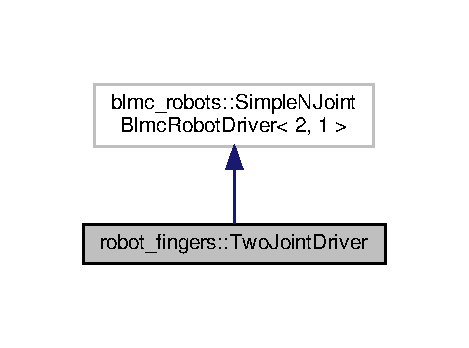
\includegraphics[width=225pt]{classrobot__fingers_1_1TwoJointDriver__inherit__graph}
\end{center}
\end{figure}


Collaboration diagram for robot\+\_\+fingers\+:\+:Two\+Joint\+Driver\+:
\nopagebreak
\begin{figure}[H]
\begin{center}
\leavevmode
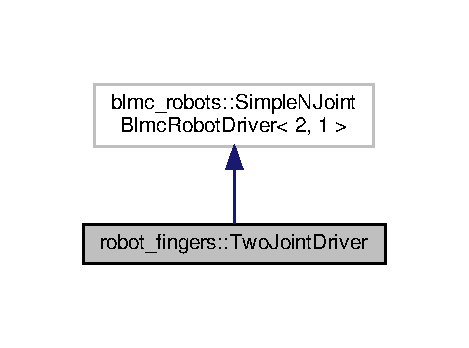
\includegraphics[width=225pt]{classrobot__fingers_1_1TwoJointDriver__coll__graph}
\end{center}
\end{figure}
\subsection*{Public Member Functions}
\begin{DoxyCompactItemize}
\item 
\mbox{\Hypertarget{classrobot__fingers_1_1TwoJointDriver_aef0955f6f1cc9f9353fb84db201aeca3}\label{classrobot__fingers_1_1TwoJointDriver_aef0955f6f1cc9f9353fb84db201aeca3}} 
{\bfseries Two\+Joint\+Driver} (const Config \&config)
\end{DoxyCompactItemize}
\subsection*{Private Member Functions}
\begin{DoxyCompactItemize}
\item 
\mbox{\Hypertarget{classrobot__fingers_1_1TwoJointDriver_a448586ec7eef35fd05352c00c87b89ff}\label{classrobot__fingers_1_1TwoJointDriver_a448586ec7eef35fd05352c00c87b89ff}} 
{\bfseries Two\+Joint\+Driver} (const Motor\+Boards \&motor\+\_\+boards, const Config \&config)
\end{DoxyCompactItemize}
\subsection*{Static Private Member Functions}
\begin{DoxyCompactItemize}
\item 
\mbox{\Hypertarget{classrobot__fingers_1_1TwoJointDriver_a3694dbc37d12ff1538aec8f3fe3e5bee}\label{classrobot__fingers_1_1TwoJointDriver_a3694dbc37d12ff1538aec8f3fe3e5bee}} 
static Motors {\bfseries create\+\_\+motors} (const Motor\+Boards \&motor\+\_\+boards)
\end{DoxyCompactItemize}


\subsection{Detailed Description}
Driver for two joints. 

Driver for a double B\+L\+MC joint. Mostly intended for testing purposes. 

The documentation for this class was generated from the following file\+:\begin{DoxyCompactItemize}
\item 
include/robot\+\_\+fingers/\hyperlink{two__joint__driver_8hpp}{two\+\_\+joint\+\_\+driver.\+hpp}\end{DoxyCompactItemize}

\chapter{File Documentation}
\hypertarget{n__finger__driver_8hpp}{}\section{include/robot\+\_\+fingers/n\+\_\+finger\+\_\+driver.hpp File Reference}
\label{n__finger__driver_8hpp}\index{include/robot\+\_\+fingers/n\+\_\+finger\+\_\+driver.\+hpp@{include/robot\+\_\+fingers/n\+\_\+finger\+\_\+driver.\+hpp}}


Driver for the Finger Robots.  


{\ttfamily \#include $<$blmc\+\_\+robots/n\+\_\+joint\+\_\+blmc\+\_\+robot\+\_\+driver.\+hpp$>$}\newline
{\ttfamily \#include $<$robot\+\_\+interfaces/finger\+\_\+types.\+hpp$>$}\newline
Include dependency graph for n\+\_\+finger\+\_\+driver.\+hpp\+:
\nopagebreak
\begin{figure}[H]
\begin{center}
\leavevmode
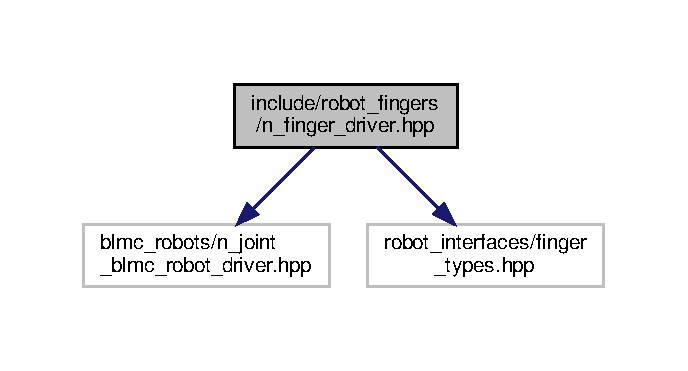
\includegraphics[width=330pt]{n__finger__driver_8hpp__incl}
\end{center}
\end{figure}
This graph shows which files directly or indirectly include this file\+:
\nopagebreak
\begin{figure}[H]
\begin{center}
\leavevmode
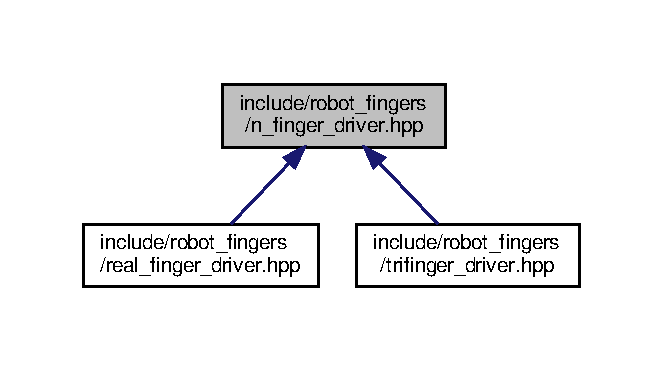
\includegraphics[width=318pt]{n__finger__driver_8hpp__dep__incl}
\end{center}
\end{figure}
\subsection*{Classes}
\begin{DoxyCompactItemize}
\item 
class \hyperlink{classrobot__fingers_1_1NFingerDriver}{robot\+\_\+fingers\+::\+N\+Finger\+Driver$<$ N\+\_\+\+F\+I\+N\+G\+E\+R\+S $>$}
\begin{DoxyCompactList}\small\item\em Driver for the Finger robots. \end{DoxyCompactList}\end{DoxyCompactItemize}


\subsection{Detailed Description}
Driver for the Finger Robots. 

\begin{DoxyCopyright}{Copyright}
2020, Max Planck Gesellschaft. All rights reserved. 
\end{DoxyCopyright}
\begin{DoxyRefDesc}{License}
\item[\hyperlink{license__license000001}{License}]B\+SD 3-\/clause \end{DoxyRefDesc}

\hypertarget{one__joint__driver_8hpp}{}\section{include/robot\+\_\+fingers/one\+\_\+joint\+\_\+driver.hpp File Reference}
\label{one__joint__driver_8hpp}\index{include/robot\+\_\+fingers/one\+\_\+joint\+\_\+driver.\+hpp@{include/robot\+\_\+fingers/one\+\_\+joint\+\_\+driver.\+hpp}}


Driver for a \char`\"{}one-\/joint\char`\"{} robot.  


{\ttfamily \#include $<$blmc\+\_\+robots/n\+\_\+joint\+\_\+blmc\+\_\+robot\+\_\+driver.\+hpp$>$}\newline
Include dependency graph for one\+\_\+joint\+\_\+driver.\+hpp\+:
\nopagebreak
\begin{figure}[H]
\begin{center}
\leavevmode
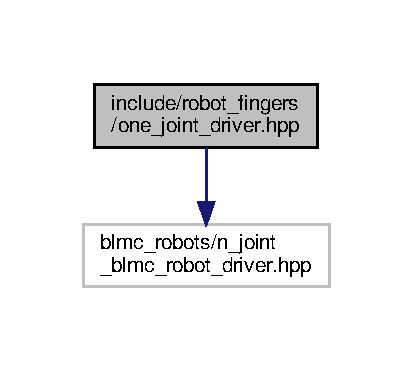
\includegraphics[width=198pt]{one__joint__driver_8hpp__incl}
\end{center}
\end{figure}
\subsection*{Classes}
\begin{DoxyCompactItemize}
\item 
class \hyperlink{classrobot__fingers_1_1OneJointDriver}{robot\+\_\+fingers\+::\+One\+Joint\+Driver}
\begin{DoxyCompactList}\small\item\em Driver for a single joint. \end{DoxyCompactList}\end{DoxyCompactItemize}


\subsection{Detailed Description}
Driver for a \char`\"{}one-\/joint\char`\"{} robot. 

\begin{DoxyCopyright}{Copyright}
Copyright (c) 2019, New York University and Max Planck Gesellschaft. 
\end{DoxyCopyright}

\hypertarget{real__finger__driver_8hpp}{}\section{include/robot\+\_\+fingers/real\+\_\+finger\+\_\+driver.hpp File Reference}
\label{real__finger__driver_8hpp}\index{include/robot\+\_\+fingers/real\+\_\+finger\+\_\+driver.\+hpp@{include/robot\+\_\+fingers/real\+\_\+finger\+\_\+driver.\+hpp}}


The hardware wrapper of the real Finger robot.  


{\ttfamily \#include \char`\"{}n\+\_\+finger\+\_\+driver.\+hpp\char`\"{}}\newline
Include dependency graph for real\+\_\+finger\+\_\+driver.\+hpp\+:
\nopagebreak
\begin{figure}[H]
\begin{center}
\leavevmode
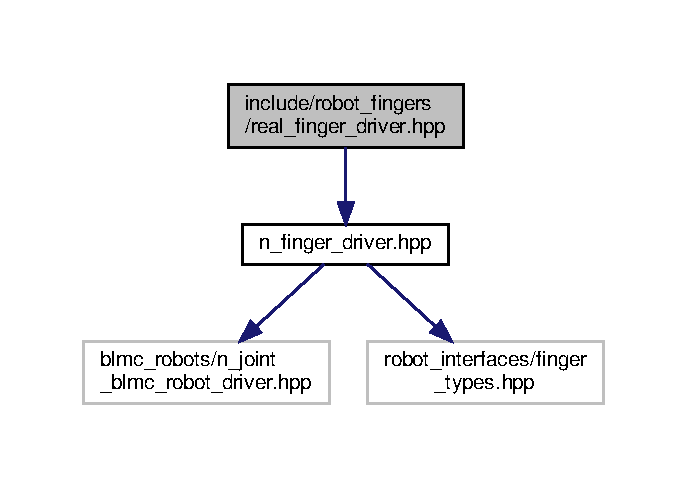
\includegraphics[width=330pt]{real__finger__driver_8hpp__incl}
\end{center}
\end{figure}
\subsection*{Classes}
\begin{DoxyCompactItemize}
\item 
class \hyperlink{classrobot__fingers_1_1RealFingerDriver}{robot\+\_\+fingers\+::\+Real\+Finger\+Driver}
\end{DoxyCompactItemize}


\subsection{Detailed Description}
The hardware wrapper of the real Finger robot. 

\begin{DoxyAuthor}{Author}
Manuel Wuthrich 
\end{DoxyAuthor}
\begin{DoxyDate}{Date}
2018 
\end{DoxyDate}
\begin{DoxyCopyright}{Copyright}
Copyright (c) 2019, New York University and Max Planck Gesellschaft. 
\end{DoxyCopyright}

\hypertarget{trifinger__driver_8hpp}{}\section{include/robot\+\_\+fingers/trifinger\+\_\+driver.hpp File Reference}
\label{trifinger__driver_8hpp}\index{include/robot\+\_\+fingers/trifinger\+\_\+driver.\+hpp@{include/robot\+\_\+fingers/trifinger\+\_\+driver.\+hpp}}


The hardware wrapper of the real Tri\+Finger robot.  


{\ttfamily \#include \char`\"{}n\+\_\+finger\+\_\+driver.\+hpp\char`\"{}}\newline
Include dependency graph for trifinger\+\_\+driver.\+hpp\+:
\nopagebreak
\begin{figure}[H]
\begin{center}
\leavevmode
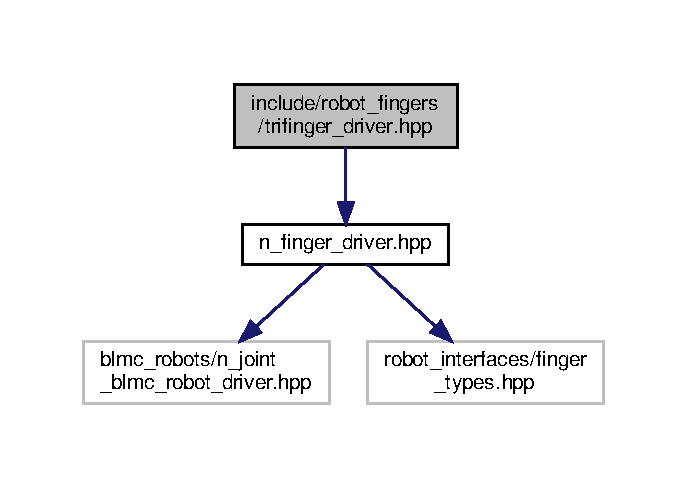
\includegraphics[width=330pt]{trifinger__driver_8hpp__incl}
\end{center}
\end{figure}
\subsection*{Classes}
\begin{DoxyCompactItemize}
\item 
class \hyperlink{classrobot__fingers_1_1TriFingerDriver}{robot\+\_\+fingers\+::\+Tri\+Finger\+Driver}
\end{DoxyCompactItemize}


\subsection{Detailed Description}
The hardware wrapper of the real Tri\+Finger robot. 

\begin{DoxyCopyright}{Copyright}
Copyright (c) 2019, New York University and Max Planck Gesellschaft. 
\end{DoxyCopyright}

\hypertarget{trifinger__platform__frontend_8hpp}{}\section{include/robot\+\_\+fingers/trifinger\+\_\+platform\+\_\+frontend.hpp File Reference}
\label{trifinger__platform__frontend_8hpp}\index{include/robot\+\_\+fingers/trifinger\+\_\+platform\+\_\+frontend.\+hpp@{include/robot\+\_\+fingers/trifinger\+\_\+platform\+\_\+frontend.\+hpp}}


Combined frontend for the Tri\+Finger Platform.  


{\ttfamily \#include $<$robot\+\_\+interfaces/finger\+\_\+types.\+hpp$>$}\newline
{\ttfamily \#include $<$robot\+\_\+interfaces/sensors/sensor\+\_\+frontend.\+hpp$>$}\newline
{\ttfamily \#include $<$trifinger\+\_\+cameras/tricamera\+\_\+observation.\+hpp$>$}\newline
{\ttfamily \#include $<$trifinger\+\_\+object\+\_\+tracking/object\+\_\+tracker\+\_\+frontend.\+hpp$>$}\newline
Include dependency graph for trifinger\+\_\+platform\+\_\+frontend.\+hpp\+:
\nopagebreak
\begin{figure}[H]
\begin{center}
\leavevmode
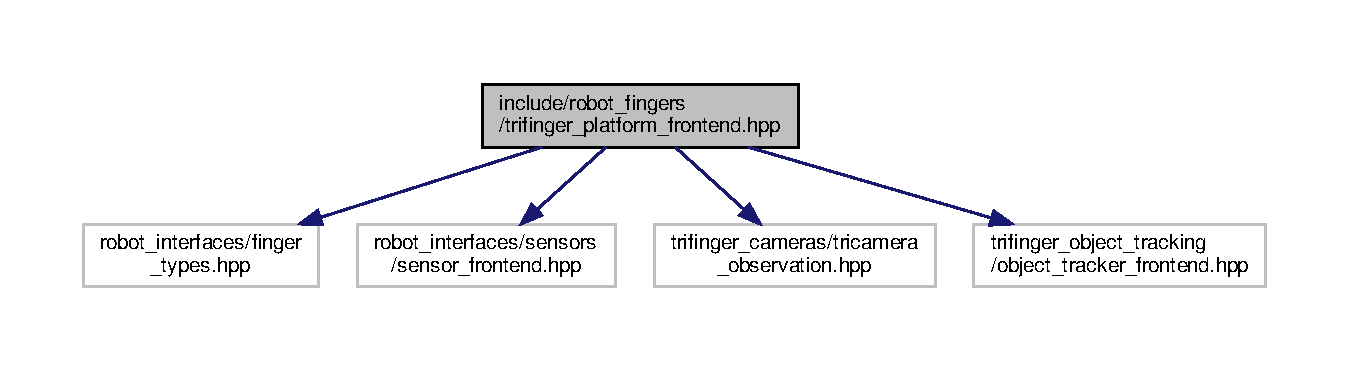
\includegraphics[width=350pt]{trifinger__platform__frontend_8hpp__incl}
\end{center}
\end{figure}
This graph shows which files directly or indirectly include this file\+:
\nopagebreak
\begin{figure}[H]
\begin{center}
\leavevmode
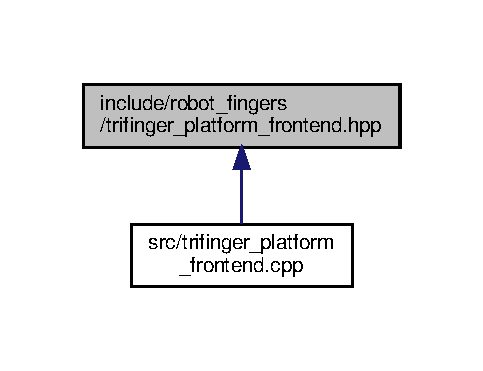
\includegraphics[width=232pt]{trifinger__platform__frontend_8hpp__dep__incl}
\end{center}
\end{figure}
\subsection*{Classes}
\begin{DoxyCompactItemize}
\item 
class \hyperlink{classrobot__fingers_1_1TriFingerPlatformFrontend}{robot\+\_\+fingers\+::\+Tri\+Finger\+Platform\+Frontend}
\begin{DoxyCompactList}\small\item\em Combined frontend for the Tri\+Finger Platform. \end{DoxyCompactList}\end{DoxyCompactItemize}


\subsection{Detailed Description}
Combined frontend for the Tri\+Finger Platform. 

\begin{DoxyCopyright}{Copyright}
2020, Max Planck Gesellschaft. All rights reserved. 
\end{DoxyCopyright}
\begin{DoxyRefDesc}{License}
\item[\hyperlink{license__license000002}{License}]B\+SD 3-\/clause \end{DoxyRefDesc}

\hypertarget{two__joint__driver_8hpp}{}\section{include/robot\+\_\+fingers/two\+\_\+joint\+\_\+driver.hpp File Reference}
\label{two__joint__driver_8hpp}\index{include/robot\+\_\+fingers/two\+\_\+joint\+\_\+driver.\+hpp@{include/robot\+\_\+fingers/two\+\_\+joint\+\_\+driver.\+hpp}}


Driver for a \char`\"{}two-\/joint\char`\"{} robot.  


{\ttfamily \#include $<$blmc\+\_\+robots/n\+\_\+joint\+\_\+blmc\+\_\+robot\+\_\+driver.\+hpp$>$}\newline
Include dependency graph for two\+\_\+joint\+\_\+driver.\+hpp\+:
\nopagebreak
\begin{figure}[H]
\begin{center}
\leavevmode
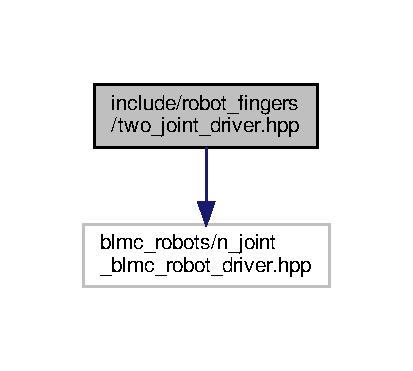
\includegraphics[width=198pt]{two__joint__driver_8hpp__incl}
\end{center}
\end{figure}
\subsection*{Classes}
\begin{DoxyCompactItemize}
\item 
class \hyperlink{classrobot__fingers_1_1TwoJointDriver}{robot\+\_\+fingers\+::\+Two\+Joint\+Driver}
\begin{DoxyCompactList}\small\item\em Driver for two joints. \end{DoxyCompactList}\end{DoxyCompactItemize}


\subsection{Detailed Description}
Driver for a \char`\"{}two-\/joint\char`\"{} robot. 

\begin{DoxyCopyright}{Copyright}
Copyright (c) 2019, New York University and Max Planck Gesellschaft. 
\end{DoxyCopyright}

\hypertarget{trifinger__platform__frontend_8cpp}{}\section{src/trifinger\+\_\+platform\+\_\+frontend.cpp File Reference}
\label{trifinger__platform__frontend_8cpp}\index{src/trifinger\+\_\+platform\+\_\+frontend.\+cpp@{src/trifinger\+\_\+platform\+\_\+frontend.\+cpp}}


Combined frontend for the Tri\+Finger Platform.  


{\ttfamily \#include $<$robot\+\_\+fingers/trifinger\+\_\+platform\+\_\+frontend.\+hpp$>$}\newline
Include dependency graph for trifinger\+\_\+platform\+\_\+frontend.\+cpp\+:
\nopagebreak
\begin{figure}[H]
\begin{center}
\leavevmode
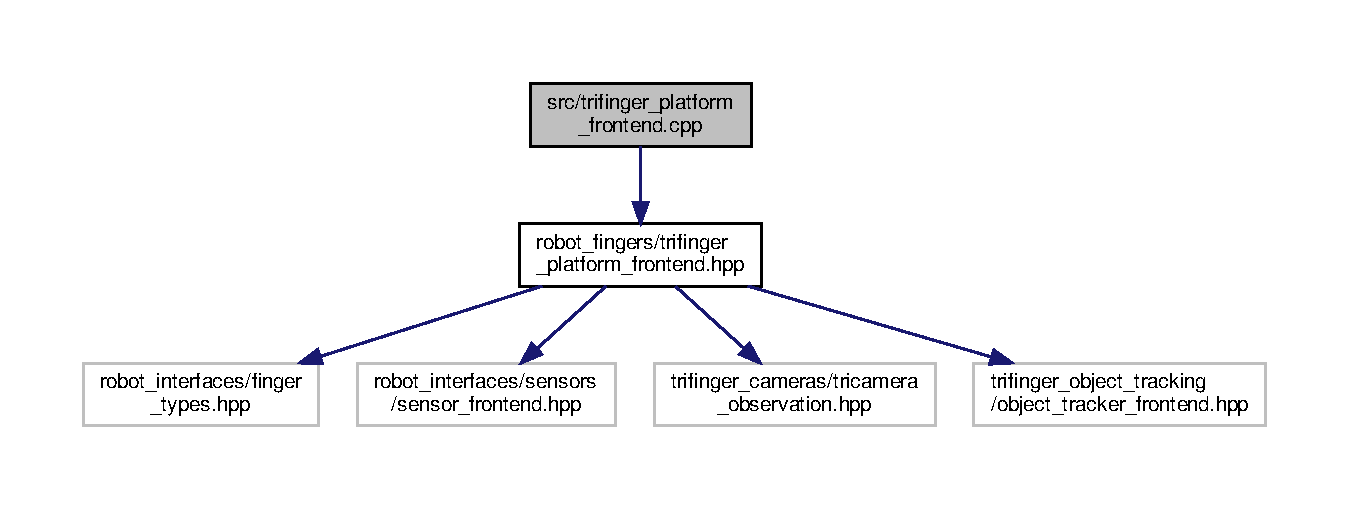
\includegraphics[width=350pt]{trifinger__platform__frontend_8cpp__incl}
\end{center}
\end{figure}


\subsection{Detailed Description}
Combined frontend for the Tri\+Finger Platform. 

\begin{DoxyCopyright}{Copyright}
2020, Max Planck Gesellschaft. All rights reserved. 
\end{DoxyCopyright}
\begin{DoxyRefDesc}{License}
\item[\hyperlink{license__license000003}{License}]B\+SD 3-\/clause \end{DoxyRefDesc}

%--- End generated contents ---

% Index
\backmatter
\newpage
\phantomsection
\clearemptydoublepage
\addcontentsline{toc}{chapter}{Index}
\printindex

\end{document}
